\documentclass{cmspaper}
\usepackage{color}
\usepackage{graphicx}
\usepackage{wrapfig}
\usepackage{slashbox}
\usepackage{epstopdf}  %added for MAC compiler
\usepackage{pdfpages}
\usepackage{appendix}
\usepackage{lineno}
\RequirePackage{lineno} 
\newcommand{\met}{\mbox{$\raisebox{.3ex}{$\not$}E_T$\hspace*{0.5ex}}}
%\newcommand{\met}{$E_{T}^{miss}$}
\newcommand{\lumi}{204~pb$^{-1}$}
\newcommand{\pt}{$p_{T}$}
\newcommand{\Ht}{$H_{T}$}
\newcommand{\ttbar}{$t\bar{t}$}
\newcommand{\ttll}{$t\bar{t}\rightarrow\ell^+\ell^-$}
\newcommand{\tttau}{$t\bar{t}\rightarrow\ell^{\pm}\tau^{\mp}/\tau^+\tau^-$}
\newcommand{\ttfake}{$t\bar{t}\rightarrow\mathrm{fake}$}
\newcommand{\wjets}{$W+\mathrm{jets}$}
\newcommand{\DY}{DY}
\newcommand{\WW}{$W^+W^-$}
\newcommand{\WZ}{$W^{\pm}Z^0$}
\newcommand{\ZZ}{$Z^0Z^0$}
\begin{document}
  
%==============================================================================
% title page for few authors

\begin{titlepage}
    \pagestyle {plain}
    \pagenumbering{arabic}
     %\linenumbers
     % select one of the following and type in the proper number:
  % \cmsnote{2010/000}
 %\date{Oct 23 16:00 PM}

  \title {Search for new physics in the opposite sign dilepton sample}
\begin{Authlist}
D. Barge, C. Campagnari, P.~Kalavase, D.~Kovalskyi, V.~Krutelyov, J.~Ribnik
\Instfoot{ucsb}{University of California, Santa Barbara}
W.~Andrews, G.~Cerati, D.~Evans, F.~Golf, J. M\"ulmenst\"adt, S. Padhi, Y.~Tu, F. W\"urthwein, A. Yagil, J.~Yoo
\Instfoot{ucsd}{University of California, San Diego}
L. Bauerdick, I.~Bloch, K.~Burkett, I.~Fisk, Y.~ Gao,~O.~Gutsche,~B. Hooberman, S.~Jindariani
\Instfoot{fnal}{Fermi National Accelerator Laboratory, Batavia, Illinois}
\end{Authlist}
 

    \begin{abstract}
We present the result of a search for new physics in the opposite-sign 
dileptons $+$ jets $+$ missing energy final state based on \lumi
of 2011 CMS data.  
%We find no evidence for an anomalous rate of events
%accompanied by large missing transverse energy and significant hadronic
%activity.

  \end{abstract}

\end{titlepage}
\newpage


\tableofcontents
\newpage
\linenumbers
\section{Changes w.r.t. previous AN Version}
\label{sec:changes}

\begin{itemize}

\item v6: Updated to full 2012 sample corresponding to 19.3 fb$^{-1}$.
\item v5: {\bf This is the version corresponding to the HCP results}. Added interpretation for the GMSB model (Sec.~\ref{sec:interpretation}). Added data vs. MC kinematic distributions for the sample with 3 leptons and at least 2 jets, where we observe an excess of data with respect to the MC prediction (App.~\ref{app:WZ}).
\item v4: Un-blinded the results of the inclusive and targeted analysis, and added an interpretation in the \wzmet\ model. Moved the material for the edge analysis to a separate AN (2012/359).
\item v3: Added results for the low-\MET\ and high-\MET\ signal regions used for the edge analysis, for the first 5.1 fb$^{-1}$ 2012A+B data.
\item v2: Updated to 9.2 fb$^{-1}$ of 53X data and MC (v1 used 5.1 fb$^{-1}$ 52X data and MC).

\end{itemize}

\section{Introduction}
\label{sec:intro}

In this note we describe a search for new physics in the 2011 
opposite sign isolated dilepton sample ($ee$, $e\mu$, and $\mu\mu$).  
The main source of 
isolated dileptons at CMS is Drell Yan and $t\bar{t}$.
Here we concentrate on dileptons with invariant mass inconsistent
with $Z \to ee$ and $Z \to \mu\mu$.  Thus $t\bar{t}$ is the most
important background.  A separate search for new physics in the $Z$ 
sample is described in a separate note\cite{ref:Ztemplates}.
This is an update of an analysis performed on 2010 data~\cite{ref:osnote,ref:ospaper}. 

The search strategy is the following

\begin{itemize}

\item We start out with a pre-selection which is as close as 
possible to the published (or soon to be published) $t\bar{t}$
dilepton analysis\cite{ref:top} (same lepton ID, same jet definitions,
etc.).  We do make a couple of substantive modifications:

\begin{enumerate}
\item The top analysis requires two leptons of $P_T > 20$ GeV.  
 In this
analysis we lower the requirement on the second lepton to $P_T > 10$ 
GeV.  This is motivated by our desire to maintain sensitivity to possible
SUSY signals with relatively low $P_T$ leptons generated in the 
cascade decays of heavy objects.
\item The top analysis requires at least two jets of $P_T > 30$
GeV with \met $>30$ GeV ($ee$ and $e\mu$) or \met $>20$ GeV ($e \mu$).
We tighten the \met cut to 50 GeV and we 
also require that the scalar sum of the $P_T$ of all jets with $P_T > 30$
GeV be $> 100$ GeV.  These requirements considerably
reduce backgrounds to the $t\bar{t}$ sample, {\em e.g.}, backgrounds
from Drell Yan and $W+$jets.
\end{enumerate}

\item The pre-selection consists mostly of $t\bar{t}$ events.  We perform 
data $-$ Monte Carlo comparisons of kinematical distributions.  Assuming
reasonable agreeement for the bulk of $t\bar{t}$ we move on to a 
search for new physics in the tail of the $t\bar{t}$.

\item Our prejudice is that new physics would manifest itself in an
excess of events with high \met and significant hadronic activity.
We define an a-priori search region by tightening the \met and 
hadronic activity requirements such that we expect of order 1\% 
of $t\bar{t}$ events to pass the selection (as predicted by Monte Carlo).

\item We perform a counting experiment in the signal region.  We compare
observed yields with expectations from Monte Carlo and with two independent
data driven techniques (see Section~\ref{sec:abcd} and~\ref{sec:victory}).

\end{itemize}





\section{Datasets}
\label{sec:datasets}

%\subsection{Datasets}

%We use a combination of rereco and prompt reco for both leptons and photons.
We use the May 10 ReReco and prompt reco data for both signal and control samples.%leptons and photons.
\\
For selecting the dilepton sample, the following datasets are used (the pythia DY samples are used only for generator level Z mass values less than 50 to avoid overlap with the madgraph DYJets sample), including the benchmark SUSY points LM4 and LM8:


\begin{itemize}
\item Data 
\begin{itemize}
\item \verb=/DoubleElectron/Run2011A-May10ReReco-v1/AOD=
\item \verb=/DoubleMu/Run2011A-May10ReReco-v1/AOD=
\item \verb=/MuEG/Run2011A-May10ReReco-v1/AOD=

\item \verb=/DoubleElectron/Run2011A-PromptReco-v4/AOD=
\item \verb=/DoubleMu/Run2011A-PromptReco-v4/AOD=
\item \verb=/MuEG/Run2011A-PromptReco-v4/AOD=
\end{itemize}

\item Monte Carlo
  \begin{itemize} 
  \item \verb=/DYJetsToLL_TuneD6T_M-50_7TeV-madgraph-tauola/Spring11-PU_S1_START311_V1G1-v1/AODSIM=
  \item \verb=/TTJets_TuneZ2_7TeV-madgraph-tauola/Spring11-PU_S1_START311_V1G1-v1/AODSIM=
  \item \verb=/WJetsToLNu_TuneZ2_7TeV-madgraph-tauola/Spring11-PU_S1_START311_V1G1-v1/AODSIM=
  \item \verb=/WWTo2L2Nu_TuneZ2_7TeV-pythia6/Spring11-PU_S1_START311_V1G1-v1/AODSIM=
  \item \verb=/WZtoAnything_TuneZ2_7TeV-pythia6-tauola/Spring11-PU_S1_START311_V1G1-v1/AODSIM=
  \item \verb=/ZZtoAnything_TuneZ2_7TeV-pythia6-tauola/Spring11-PU_S1_START311_V1G1-v1/AODSIM=
  \item \verb=/TToBLNu_TuneZ2_s-channel_7TeV-madgraph/Spring11-PU_S1_START311_V1G1-v1/AODSIM=
  \item \verb=/TToBLNu_TuneZ2_t-channel_7TeV-madgraph/Spring11-PU_S1_START311_V1G1-v1/AODSIM=
  \item \verb=/TToBLNu_TuneZ2_tW-channel_7TeV-madgraph/Spring11-PU_S1_START311_V1G1-v1/AODSIM=
  \item Pythia samples:
  \item \verb=/DYToEE_M-20_CT10_TuneZ2_7TeV-powheg-pythia/Spring11-PU_S1_START311_V1G1-v1/AODSIM=
  \item \verb=/DYToMuMu_M-20_CT10_TuneZ2_7TeV-powheg-pythia/Spring11-PU_S1_START311_V1G1-v1/AODSIM=
  \item \verb=/DYToTauTau_M-20_CT10_TuneZ2_7TeV-powheg-pythia-tauola/Spring11-PU_S1_START311_V1G1-v1/AODSIM=
  \item \verb=/DYToEE_M-10To20_TuneZ2_7TeV-pythia6/Spring11-PU_S1_START311_V1G1-v1/AODSIM=
  \item \verb=/DYToMuMu_M-10To20_TuneZ2_7TeV-pythia6/Spring11-PU_S1_START311_V1G1-v1/AODSIM=
  \item LM samples:
  \item \verb=/LM4_SUSY_sftsht_7TeV-pythia6/Spring11-PU_S1_START311_V1G1-v1/AODSIM=
  \item \verb=/LM8_SUSY_sftsht_7TeV-pythia6/Spring11-PU_S1_START311_V1G1-v1/AODSIM=
  \end{itemize}
\end{itemize}

For the creation of photon templates, we use:

\begin{itemize}
\item \verb=/Photon/Run2011A-May10ReReco-v1/AOD=
\item \verb=/Photon/Run2011A-PromptReco-v4/AOD=
%\item \verb==
\end{itemize}

The integrated luminosity used corresponds to \lumi, and the JSON used is 
the official May 10 ReReco 
and July 1 prompt reco
JSON:
\\
Cert\_160404-163869\_7TeV\_May10ReReco\_Collisions11\_JSON.txt
%Cert_160404-163869_7TeV_May10ReReco_Collisions11_JSON.txt
\\
Cert\_160404-167784\_7TeV\_PromptReco\_Collisions11\_JSON.txt
%Cert_160404-167784_7TeV_PromptReco_Collisions11_JSON.txt

\section{Event Preselection}
\label{sec:eventSel}
The purpose of the preselection is to reject backgrounds other than 
$t\bar{t} \to$ dileptons.  We compare the kinematical 
properties of this sample with expectations from $t\bar{t}$ 
Monte Carlo.

The preselection is based on the 
$t\bar{t}$ analysis~\cite{ref:top}.  
We select events with two opposite sign, well-identified and isolated
leptons ($ee$, $e\mu$, or $\mu\mu$); one of the leptons must 
have $P_T > 20$ GeV,
the other one must have $P_T > 10$ GeV. Events with dilepton mass
consistent with $Z \to ee/\mu\mu$ are rejected.
In case of events with 
more than two such leptons, we select the pair that maximizes the scalar 
sum of lepton $P_T$'s.
There must be at least two 
pfjets of $P_T > 30$ GeV and $|\eta| < 3.0$;  jets must pass
loose {\tt pfJetId} and be separated by $\Delta R >$ 0.4 from any 
lepton with $P_T > 10$~GeV passing the selection.
The scalar sum \Ht\ of the 
$P_T$ of all such jets must exceed 100 GeV, for the dilepton-\Ht\ sample
this requirement is increased to 200 GeV since these triggers have large inefficiency
below this threshold.
Finally $\met > 50$ GeV (we use pfmet). More details are given in the subsections below.

\subsection{Event Cleanup}
\label{sec:cleanup}

\begin{itemize}
   \item Require at least one good deterministic annealing (DA) vertex
   \begin{itemize}
      \item not fake
      \item ndof $>$ 4
      \item $|\rho| < 2$ cm
      \item $|z| < 24$ cm.  
   \end{itemize}
\end{itemize}


\subsection{Muon Selection}
\label{sec:muon}

Muon candidates are RECO muon objects passing the following
requirements:

\begin{itemize}

\item $p_{T} > 5$~GeV and $|\eta| < 2.4$

\item Global Muon and Tracker Muon

\item $\chi^2$/ndof of global fit $<$ 10

\item At least 11 hits in the tracker fit

\item Impact parameter with respect to the first DA vertex $d_{0} < 200$~$\mu$m and $d_{z} < 1$~cm

\item $Iso \equiv E_T^{\rm iso}/p_T < $~0.15, $E_T^{\rm iso}$ is defined as the sum of 
transverse energy/momentum deposits in ecal, hcal, and tracker, in a cone of 0.3

\item At least one of the hits from the 
standalone muon must be used in the global fit

\item Require tracker $\Delta p_T/p_T < 0.1$. This cut was not in the original top analysis.
It is motivated by the observation of poorly measured muons in data with large
relative $p_T$ uncertainty, giving significant contributions to the \met

\item {\color{red} \bf LIST FO DEFINITIONS HERE? }

\end{itemize}



\subsection{Electron Selection}
\label{sec:electron}

Electron candidates are RECO GSF electrons passing the following requirements:

\begin{itemize}

\item $p_{T}>10$~GeV and $|\eta| < 2.5$.

\item Veto electrons with a supercluster in the transition region $1.4442 < |\eta| < 1.556$.

\item VBTF90 identification\cite{ref:vbtf} with requirements tightened to match the CaloIdT and TrkIdVL HLT requirements:

  \begin{itemize}
  \item $\sigma_{i\eta i\eta} < $ 0.01 (EB), 0.03 (EE)
  \item $\Delta\phi < $ 0.15 (EB), 0.10 (EE)
  \item $\Delta\eta < $ 0.007 (EB), 0.009 (EE)
  \item $H/E < $ 0.1 (EB), 0.075 (EE)
  \end{itemize}  

\item Impact parameter with respect to the first DA vertex $d_0 < 400$~$\mu$m and $d_z < 1$~cm.

\item $Iso \equiv $ $E_T^{\rm iso}/p_T < $ 0.15.  $E_T^{\rm iso}$
is defined as the sum of transverse energy/momentum deposits in ecal,
hcal, and tracker, in a 
cone of 0.3.  A 1 GeV pedestal is subtracted from the ecal energy 
deposition in the EB, however the ecal energy is never allowed to 
go negative.

\item Electrons with a tracker or global muon within $\Delta R$ of 
0.1 are vetoed.

\item The number of missing expected inner hits must be less than 
two~\cite{ref:conv}.

\item Conversion removal via partner track finding: any electron
where an additional GeneralTrack is found with $Dist < 0.02$ cm 
and $\Delta \cot \theta < 0.02$ is vetoed~\cite{ref:conv}.

%\item Cleaning for ECAL spike (aka Swiss-Cross cleaning) has been applied
%at the reconstruction level (CMSSW 38x).

\item {\color{red} \bf LIST FO DEFINITIONS HERE? }

\end{itemize}

\subsection{Invariant mass requirement}
\label{sec:zveto}

We remove $e^+e^-$ and $\mu^+ \mu^-$ events with invariant 
mass between 76 and 106 GeV.  We also remove events
with invariant mass $<$ 12 GeV, since this kinematical region is 
not well reproduced in CMS Monte Carlo and to remove Upsilons.

In addition, we remove $Z \to \mu\mu\gamma$
candidates with the $\gamma$ collinear with one of the muons.  This is
done as follows:
if the ecal energy associated with one of the muons is greater than 6 GeV,
we add this energy to the momentum of the initial muon, and we recompute
the $\mu\mu$ mass.  If this mass is between 76 and 106 GeV, the event is rejected.


\subsection{Trigger Selection}
\label{sec:trigSel}

We do not make any requirements on HLT bits in the Monte Carlo.
Instead, as discussed in 
Section~\ref{sec:trgEff}, a trigger efficiency weight is applied
to each event, based on the trigger efficiencies measured on data (see Sec.~\ref{sec:trgEff}).

We select data events using the following triggers. An event in the $ee$ channel is required
to pass a DoubleElectron trigger, an event in the $\mu\mu$ channel is required to pass a 
DoubleMu trigger, and an event in the $e\mu$ channel is required to pass a Ele-Mu trigger.

   \begin{itemize}
      \item High \pt\ dilepton trigger sample
      \begin{itemize}
         \item \verb=HLT_Ele17_CaloIdL_CaloIsoVL_Ele8_CaloIdL_CaloIsoVL=
         \item {\footnotesize \verb=HLT_Ele17_CaloIdT_TrkIdVL_CaloIsoVL_TrkIsoVL_Ele8_CaloIdT_TrkIdVL_CaloIsoVL_TrkIsoVL=}
         \item \verb=HLT_DoubleMu7=
         \item \verb=HLT_Mu13_Mu7=
         \item \verb=HLT_Mu17_Ele8_CaloIdL=
         \item \verb=HLT_Mu8_Ele17_CaloIdL=
      \end{itemize}
      \item Lepton \Ht\ cross trigger sample
      \begin{itemize}
        \item \verb=HLT_DoubleMu3_HT150=
        \item \verb=HLT_DoubleMu3_HT160=
        \item \verb=HLT_Mu3_Ele8_CaloIdL_TrkIdVL_HT150=
        \item \verb=HLT_Mu3_Ele8_CaloIdT_TrkIdVL_HT150=
        \item \verb=HLT_Mu3_Ele8_CaloIdL_TrkIdVL_HT160=
        \item \verb=HLT_Mu3_Ele8_CaloIdT_TrkIdVL_HT160=
        \item \verb=HLT_DoubleEle8_CaloIdL_TrkIdVL_HT150=
        \item \verb=HLT_DoubleEle8_CaloIdT_TrkIdVL_HT150=
        \item \verb=HLT_DoubleEle8_CaloIdL_TrkIdVL_HT160=
        \item \verb=HLT_DoubleEle8_CaloIdT_TrkIdVL_HT160=
      \end{itemize}
   \end{itemize}









\section{Trigger efficiency}
\label{sec:trgEff}

The DoubleElectron triggers have an efficiency which is close to 100\%. However, the efficiency for a single
leg to pass the muon trigger is approximately 95\% ({\color{red} \bf NEED A REF OR SOME PLOTS IN BACKUP FOR THIS}),
causing the DoubleMu (El-Mu) triggers to have an efficiency of approximately 90\% (95\%). Unless otherwise
specified, these trigger efficiencies are applied to the MC. 
{\color{red} \bf IS THIS SUFFICIENT? DO WE WANT A MORE DETAILED TRIG EFFICIENCY MODEL, OR MORE ACCURATE TRIG EFFICIENCIES?}


{\color{red} \bf WILL ADD HT TURN ON CURVES HERE.}



%\section{Preselection yields}
%\label{sec:yields}

The data yields and corresponding MC predictions after this event preselection
are given in Table~\ref{tab:yields}. The MC yields are normalized to~\lumifinal\ using 
next-to-leading order (NLO) cross sections. At the current LHC luminosity, the mean
number of interactions in a single beam crossing is approximately 5. In the MC, multiple interactions
are superimposed on the hard collision, and the MC is reweighted such that the distribution
of reconstructed primary vertices matches that in data. As expected, the MC predicts that the 
sample passing the preselection is dominated by dilepton $t\bar{t}$. The data yield is in 
reasonable agreement~\footnote{The luminosity is currently underestimated by approximately 10\%,
which explains the observed excess in data. The estimate will be updated before EPS.}
 with the prediction. We also quote the yields for
the LM1 and LM3 benchmark scenarios.

\begin{table}[htb]
\begin{center}
\caption{\label{tab:yields} Data yields and MC predictions after preselection, using the quoted NLO production cross sections $\sigma$.
The \ttll\ corrresponds  to dilepton $t\bar{t}$, including 
$t \to W \to \tau \to \ell$; \ttfake\ includes all other $t\bar{t}$ decay modes. 
The samples of MC $t\bar{t}$, $W^{\pm}$ + jets, and single-top events were 
generated with \MADGRAPH. The Drell--Yan sample (which includes events with
invariant masses as low as 10\GeVcc) was generated using a mixture of \MADGRAPH\ and 
\PYTHIA  and includes decays to the $\tau^+\tau^-$ final state. All other samples were generated with \PYTHIA. 
The LM1 and LM3 benchmark scenarios are defined in the text; the quoted $\sigma$ values refer to the total production
cross section for SUSY particles in these scenarios. Uncertainties are statistical only.
}
\vspace{2 mm}
\begin{tabular}{lr|cccc}
\hline
         Sample     & $\sigma$ [pb]  &            $ee$   &       $\mu\mu$   &         $e\mu$   &       total  \\
\hline
          \ttll     &     17 & 147.6 $\pm$ 3.2   &166.4 $\pm$ 3.2   &391.7 $\pm$ 5.1   &705.8 $\pm$ 6.8  \\
        \ttfake     &    141 &   4.5 $\pm$ 0.6   &  1.3 $\pm$ 0.3   &  8.1 $\pm$ 0.7   & 13.9 $\pm$ 1.0  \\
DY$\to\ell^+\ell^-$ &  16677 &   6.6 $\pm$ 1.8   &  9.5 $\pm$ 2.1   & 13.4 $\pm$ 2.6   & 29.6 $\pm$ 3.8  \\
            \WW     &     43 &   1.4 $\pm$ 0.2   &  1.5 $\pm$ 0.2   &  3.4 $\pm$ 0.2   &  6.3 $\pm$ 0.3  \\
            \WZ     &     18 &   0.3 $\pm$ 0.0   &  0.4 $\pm$ 0.0   &  0.7 $\pm$ 0.1   &  1.3 $\pm$ 0.1  \\
            \ZZ     &    5.9 &   0.1 $\pm$ 0.0   &  0.1 $\pm$ 0.0   &  0.2 $\pm$ 0.0   &  0.4 $\pm$ 0.0  \\
     single top     &    102 &   4.5 $\pm$ 0.2   &  5.0 $\pm$ 0.2   & 11.9 $\pm$ 0.3   & 21.4 $\pm$ 0.5  \\
         \wjets     &  96648 &   4.5 $\pm$ 1.9   &  0.0 $\pm$ 0.0   &  2.8 $\pm$ 1.7   &  7.3 $\pm$ 2.6  \\
\hline
    total SM MC     &        & 169.7 $\pm$ 4.2   &184.3 $\pm$ 3.9   &432.2 $\pm$ 6.0   &786.1 $\pm$ 8.3  \\
\hline
           data     &        &             193   &            201   &            485   &            879  \\
\hline
            LM1     &    6.7 &  22.3 $\pm$ 0.6   & 24.8 $\pm$ 0.6   & 12.8 $\pm$ 0.4   & 59.9 $\pm$ 0.9  \\
            LM3     &    5.3 &   7.9 $\pm$ 0.3   &  9.6 $\pm$ 0.3   & 14.2 $\pm$ 0.4   & 31.7 $\pm$ 0.6  \\
\hline
\end{tabular}
\end{center}
\end{table}


\section{Properties of data passing the preselection}
\label{sec:bulk}
A number of kinematical distributions for events passing 
the preselection in data are compared with MC in 
Appendix~\ref{sec:appendix}.  We find that
the MC does a good job of reproducing the properties of 
the bulk of $t\bar{t} \to $ dilepton events.  Therefore
we turn our attention to the tails of the $t\bar{t}$ 
events. 
%\section{Definition of the signal regions}
\label{sec:sigregion}

We define signal regions to look for possible
new physics contributions by adding the requirement of large MET to the preselection. Our choice of MET requirements 
to define the signal regions is driven by the MET distributions expected from $Z$ and $t\bar{t}$ MC, as shown in Fig.~\ref{fig:metdist}.

\begin{figure}[tbh]
\begin{center}
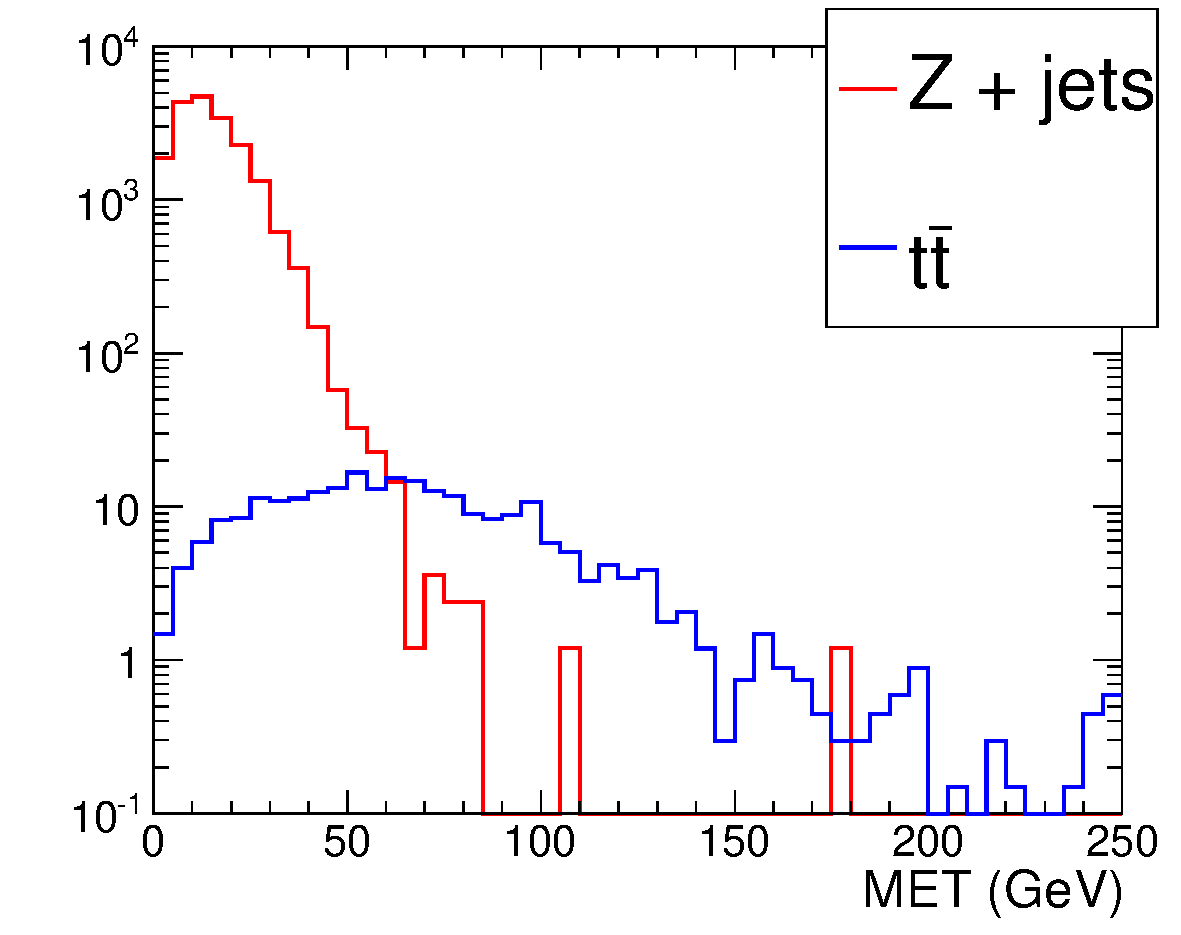
\includegraphics[width=0.75\linewidth]{plots/met_ttbar_Z.pdf}
\caption{\label{fig:metdist}\protect Distributions of MET in $Z$ and $t\bar{t}$ MC normalized to \lumi.}
\end{center}
\end{figure}

We define two signal regions for our search:
\begin{itemize}
\item MET $>$ 60 GeV (loose signal region):
In this region of MET there is a contribution from the tail of the MET distribution 
in \Z plus jets events. There is also a contribution from \ttbar events where the leptons happen to be in the \Z 
mass window. 
%We expect the MC simulation to do a good job on the second source, as it is well within the 
%bulk of the \ttbar phase space. However, for the first we must rely on data driven procedures. 

The MC and data yields for this signal region are given in Table~\ref{sigyieldtable60} and the dilepton
mass distributions are shown in Fig.~\ref{fig:dilmass60}.

More information on the data events in this signal region is given in Table~\ref{sig60events} and information 
on the muons in these events is given in Table~\ref{sig60muons}.

\item MET $>$ 120 GeV (tight signal region):
This signal region was selected by picking a region where the SM prediction 
for the dataset we have is  $\approx$ 1 event. 
At this kinematical region the dominant background contribution is expected to be from \ttbar.

The MC and data yields for this signal region are given in Table~\ref{sigyieldtable120}.
\end{itemize}

\noindent The data driven technique used to predict the missing transverse energy accompanying 
a \Z event is described in Section~\ref{sec:templates}.

\noindent To estimate the \ttbar background we will use the opposite flavor subtraction
 described in Section~\ref{sec:topbkg}.


\begin{figure}[hbt]
\begin{center}
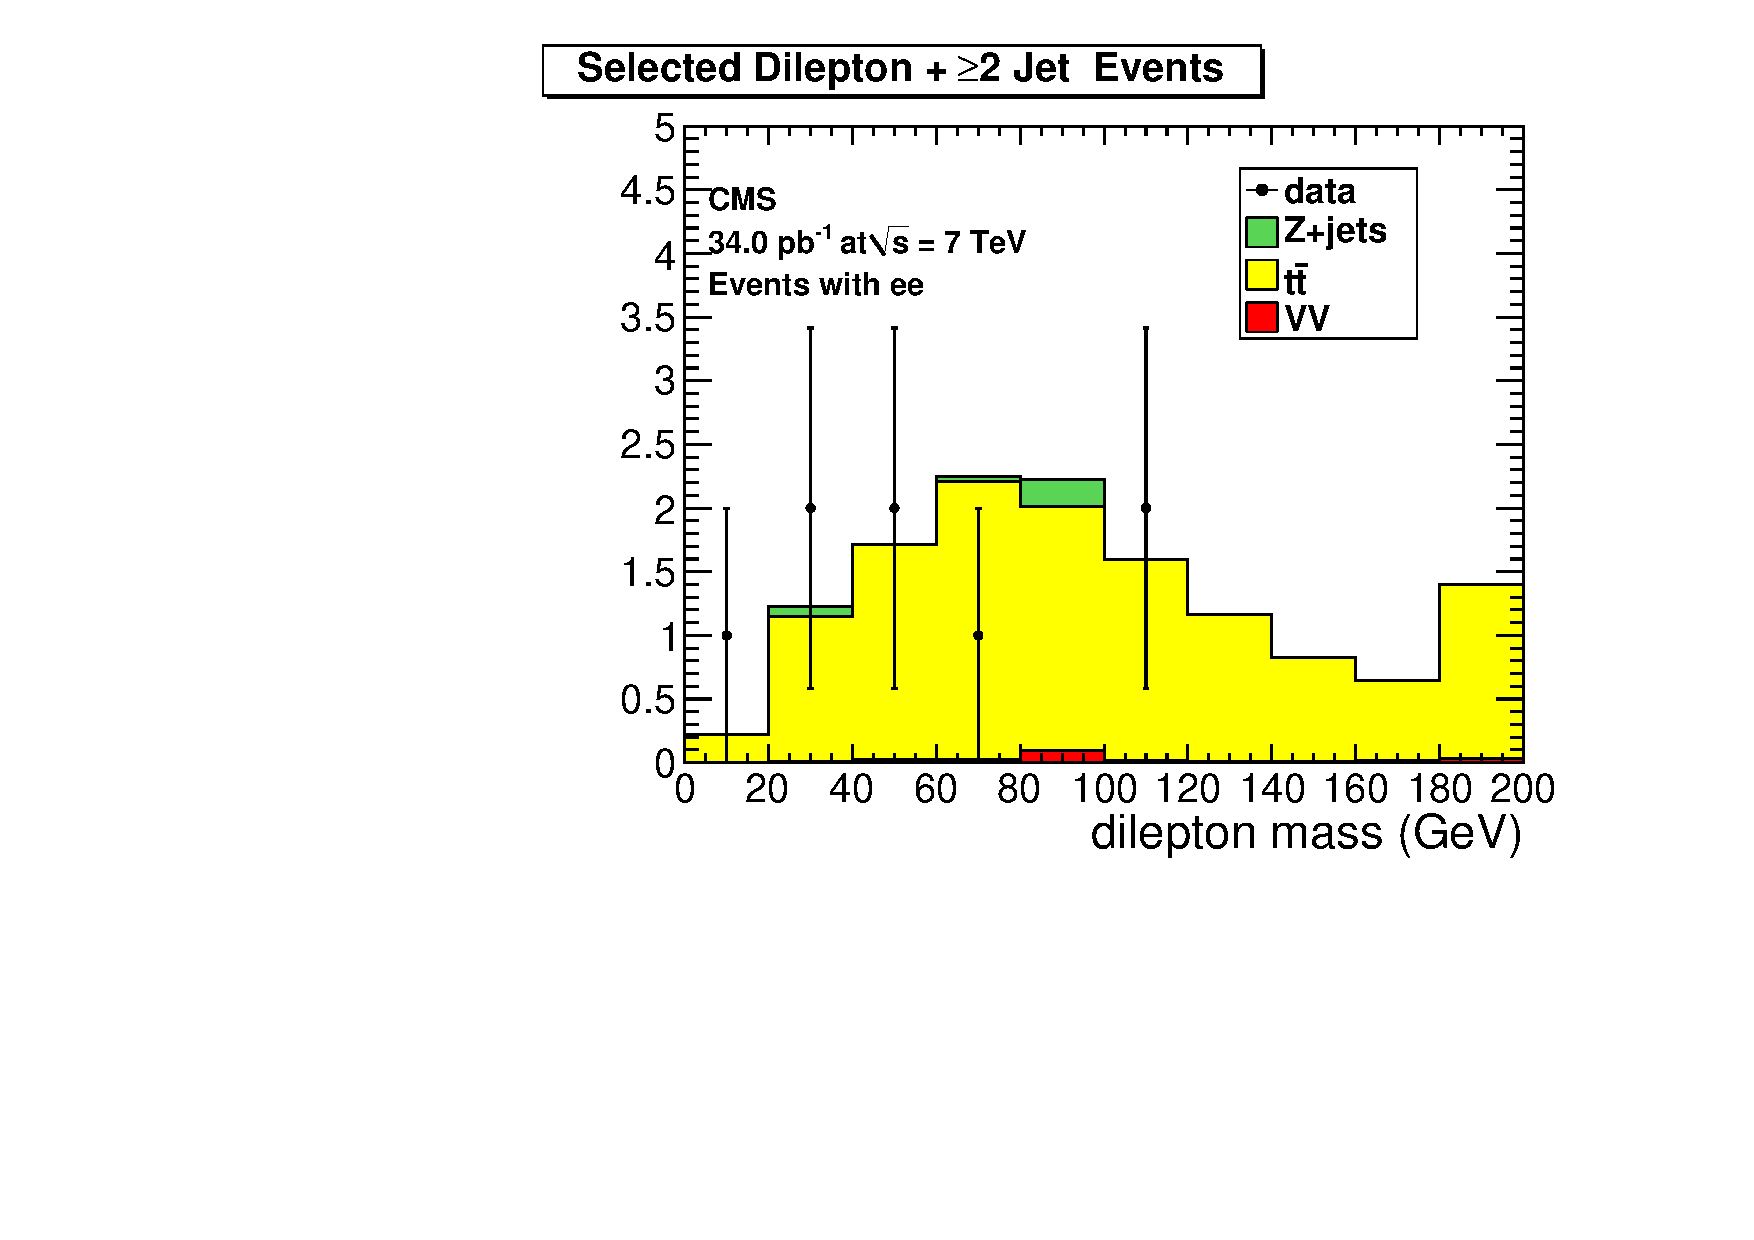
\includegraphics[width=0.48\linewidth]{plots/hdilmass_pfmet60_ee_allj.pdf}
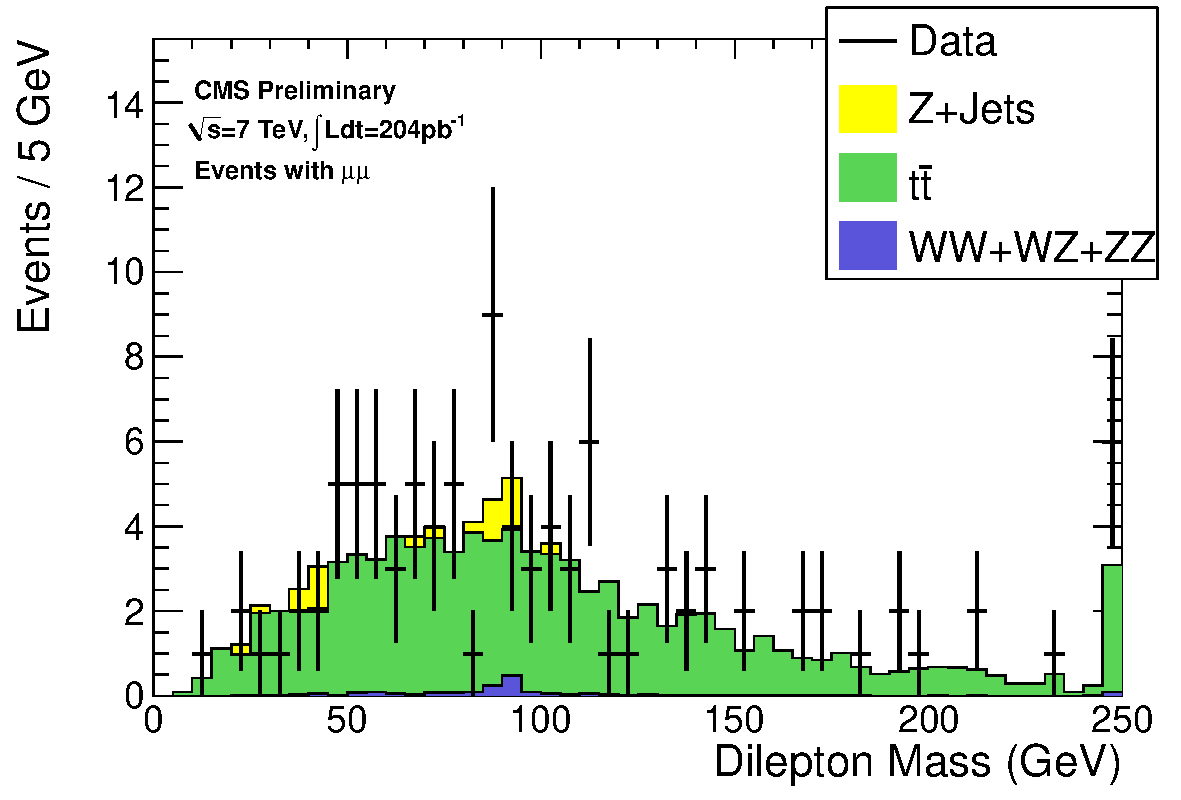
\includegraphics[width=0.48\linewidth]{plots/hdilmass_pfmet60_mm_allj.pdf}
\caption{\label{fig:dilmass60}\protect Dilepton mass distribution for events passing the pre-selection 
  and MET $>$ 60~GeV for \lumi\ in the $ee$ (left) and $\mu\mu$ (right) final states. Backgrounds from single top 
  and $W$+jets are omitted since they are negligible.}
\end{center}
\end{figure}

\begin{table}[htb]
\begin{center}
\caption{\label{sigyieldtable60} Data and Monte Carlo yields for the loose signal region MET $>$ 60~GeV  for \lumi.}
\begin{tabular}{lccccc}
%%%official PVT json v3, 38X MC 
\hline
              Sample   &                $ee$   &            $\mu\mu$   &              $e\mu$   &                 tot  \\
\hline
               ZJets   &     0.21 $\pm$ 0.09   &     0.21 $\pm$ 0.09   &     0.04 $\pm$ 0.04   &     0.46 $\pm$ 0.14  \\
               TTbar   &     1.89 $\pm$ 0.09   &     2.04 $\pm$ 0.09   &     4.17 $\pm$ 0.13   &     8.11 $\pm$ 0.18  \\
               WJets   &     0.00 $\pm$ 0.00   &     0.00 $\pm$ 0.00   &     0.00 $\pm$ 0.00   &     0.00 $\pm$ 0.00  \\
                  WW   &     0.01 $\pm$ 0.00   &     0.02 $\pm$ 0.00   &     0.03 $\pm$ 0.01   &     0.06 $\pm$ 0.01  \\
                  WZ   &     0.06 $\pm$ 0.00   &     0.06 $\pm$ 0.00   &     0.00 $\pm$ 0.00   &     0.12 $\pm$ 0.00  \\
                  ZZ   &     0.03 $\pm$ 0.00   &     0.03 $\pm$ 0.00   &     0.00 $\pm$ 0.00   &     0.06 $\pm$ 0.00  \\
                  tW   &     0.06 $\pm$ 0.01   &     0.06 $\pm$ 0.01   &     0.14 $\pm$ 0.01   &     0.26 $\pm$ 0.01  \\
\hline
           tot SM MC   &     2.26 $\pm$ 0.13   &     2.43 $\pm$ 0.13   &     4.39 $\pm$ 0.13   &     9.07 $\pm$ 0.22  \\
\hline
                data   &                   0   &                   7   &                   3   &                  10  \\
\hline
                 LM4   &     0.42 $\pm$ 0.01   &     0.44 $\pm$ 0.01   &     0.07 $\pm$ 0.01   &     0.93 $\pm$ 0.02  \\
                 LM8   &     0.19 $\pm$ 0.01   &     0.22 $\pm$ 0.01   &     0.07 $\pm$ 0.00   &     0.48 $\pm$ 0.01  \\
\hline
\end{tabular}
\end{center}
\end{table}



\begin{table}[htb]
\begin{center}
\caption{\label{sig60events} Details of data events for the loose signal region MET $>$ 60~GeV for \lumi. 
All 7 events are in the $\mu\mu$ final states. The SimpleSecondaryVertexTagger high efficiency medium 
working point is used for b-tagging, for which the efficiency is $\sim40$\% and the mistag rate is $\sim1$\%.}
\begin{tabular}{rrrrrrrrrr}

\hline

Run & Lumi & Event & Njet & N B Tag & pfMET & tcMET & Dilep Mass & Sum & Z \pt\\
 &  Section &  &  &  &  &  &  & jet \pt &  \\
\hline
147216 & 48 & 35885648 & 2 & 0 & 78.9 & 72.9 & 95.0 & 216.4 & 116.4\\
147217 & 75 & 55188718 & 2 & 0 & 79.7 & 67.8 & 90.7 & 75.7 & 39.1\\
147450 & 82 & 29253181 & 5 & 0 & 63.6 & 70.8 & 97.9 & 429.5 & 312.0\\
148862 & 350 & 522383338 & 4 & 1 & 90.0 & 75.7 & 82.4 & 373.4 & 87.0\\
149181 & 1769 & 1675896175 & 2 & 1 & 67.8 & 64.4 & 97.2 & 163.9 & 128.6\\
149291 & 205 & 199787369 & 4 & 0 & 74.5 & 92.9 & 85.0 & 303.1 & 64.3\\
149291 & 232 & 235101408 & 2 & 1 & 87.3 & 90.0 & 88.7 & 315.4 & 32.4\\

\hline
\end{tabular}
\end{center}
\end{table}


\begin{table}[htb]
\begin{center}
\caption{\label{sig60muons} Details of the muons in events in the loose signal region MET $>$ 60~GeV for \lumi. 
Shown are the transverse momentum, the relative error in the transverse momentum, d0 calculated with respect to the beamspot,
the number of hits in the Silicon track, the number of layers crossed by the Silicon track, the normalized $\chi^2$,
whether a muon segment was found in the last chamber traversed by the muon, and the number of hits in the muon chambers used in the global fit. }
\begin{tabular}{rrrrrrrrrr}
\hline

Event & Si \pt &  Si \pt & gfit \pt & d0 & N Si Hits & N Si & Si $\chi^2$ & TMLast & gfit STA \\
 &  &  rel err &  &  &  &  Layers &  & Station & hits \\
 &  &  &  &  &  &  &  & Loose &  \\
\hline
35885648 & 110.2 & 0.030 & 111.3 & -0.001 & 29 & 15 & 0.65 & 1 & 18 \\
35885648 & 27.5 & 0.012 & 27.5 & 0.005 & 16 & 12 & 0.26 & 1 & 18 \\
55188718 & 22.4 & 0.017 & 22.4 & -0.003 & 15 & 10 & 0.93 & 1 & 25 \\
55188718 & 46.7 & 0.016 & 46.9 & 0.007 & 19 & 13 & 0.79 & 1 & 35 \\
29253181 & 71.2 & 0.026 & 70.5 & -0.011 & 25 & 15 & 0.78 & 1 & 13 \\
29253181 & 255.7 & 0.068 & 301.0 & -0.011 & 24 & 15 & 0.69 & 1 & 13 \\
522383338 & 89.1 & 0.018 & 89.4 & -0.000 & 16 & 12 & 0.43 & 1 & 26 \\
522383338 & 27.1 & 0.011 & 27.1 & -0.004 & 16 & 12 & 0.13 & 1 & 36 \\
1675896175 & 80.3 & 0.017 & 80.1 & 0.002 & 19 & 13 & 0.60 & 1 & 32 \\
1675896175 & 77.6 & 0.016 & 77.5 & -0.000 & 17 & 13 & 0.21 & 1 & 25 \\
199787369 & 22.6 & 0.018 & 22.5 & -0.000 & 21 & 14 & 0.59 & 1 & 12 \\
199787369 & 82.0 & 0.033 & 80.9 & -0.002 & 12 & 10 & 0.61 & 1 & 14 \\
235101408 & 30.6 & 0.014 & 30.9 & -0.007 & 16 & 11 & 0.14 & 1 & 29 \\
235101408 & 59.7 & 0.013 & 59.9 & 0.006 & 20 & 13 & 0.37 & 1 & 16 \\


\hline
\end{tabular}
\end{center}
\end{table}



\begin{table}[htb]
\begin{center}
\caption{\label{sigyieldtable120} Data and Monte Carlo yields for the loose signal region MET $>$ 120~GeV  for \lumi.}
\begin{tabular}{lccccc}
%%%official PVT json v3, 38X MC
\hline
              Sample   &                $ee$   &            $\mu\mu$   &              $e\mu$   &                 tot  \\
\hline
               ZJets   &     0.00 $\pm$ 0.00   &     0.00 $\pm$ 0.00   &     0.00 $\pm$ 0.00   &     0.00 $\pm$ 0.00  \\
               TTbar   &     0.26 $\pm$ 0.03   &     0.28 $\pm$ 0.03   &     0.55 $\pm$ 0.05   &     1.09 $\pm$ 0.06  \\
               WJets   &     0.00 $\pm$ 0.00   &     0.00 $\pm$ 0.00   &     0.00 $\pm$ 0.00   &     0.00 $\pm$ 0.00  \\
                  WW   &     0.00 $\pm$ 0.00   &     0.00 $\pm$ 0.00   &     0.00 $\pm$ 0.00   &     0.01 $\pm$ 0.00  \\
                  WZ   &     0.01 $\pm$ 0.00   &     0.01 $\pm$ 0.00   &     0.00 $\pm$ 0.00   &     0.02 $\pm$ 0.00  \\
                  ZZ   &     0.01 $\pm$ 0.00   &     0.01 $\pm$ 0.00   &     0.00 $\pm$ 0.00   &     0.02 $\pm$ 0.00  \\
                  tW   &     0.00 $\pm$ 0.00   &     0.01 $\pm$ 0.00   &     0.02 $\pm$ 0.00   &     0.03 $\pm$ 0.00  \\
\hline
           tot SM MC   &     0.29 $\pm$ 0.03   &     0.31 $\pm$ 0.03   &     0.58 $\pm$ 0.05   &     1.17 $\pm$ 0.07  \\
\hline
                data   &                   0   &                   0   &                   0   &                   0  \\
\hline
                 LM4   &     0.33 $\pm$ 0.01   &     0.35 $\pm$ 0.01   &     0.06 $\pm$ 0.01   &     0.74 $\pm$ 0.02  \\
                 LM8   &     0.14 $\pm$ 0.01   &     0.16 $\pm$ 0.01   &     0.06 $\pm$ 0.00   &     0.36 $\pm$ 0.01  \\
\hline
\end{tabular}
\end{center}
\end{table}


%\section{Counting Experiments}
\label{sec:datadriven}

To look for possible BSM contributions, we define 2 signal regions that reject all but
0.1\% of the dilepton $t\bar{t}$ events, by adding requirements of large \MET\ and \Ht:

\begin{itemize}
\item high \MET\ signal region: \MET\ $>$ 275~GeV, \Ht\ $>$ 300~GeV,
\item high \Ht\ signal region:  \MET\ $>$ 200~GeV, \Ht\ $>$ 600~GeV.
\end{itemize}

For the high \MET\ (high \Ht) signal region, the MC predicts 2.6 (2.5) SM events, 
dominated by dilepton $t\bar{t}$; the expected LM1 yield is 17 (14) and the
expected LM3 yield is 6.4 (6.7). The signal regions are indicated in Fig.~\ref{fig:met_ht}.
These signal regions are tighter than the one used in our published 2010 analysis since 
with the larger data sample they allow us to explore phase space farther from the core
of the SM distributions.


We perform counting experiments in these signal regions, and use three independent methods to estimate from data the background in the signal region.
The first method is a novel technique which is a variation of the ABCD method, which we used in our 2010 analysis~\cite{ref:ospaper}, 
and exploits the fact that \HT\ and $y \equiv \MET/\sqrt{H_T}$ are nearly uncorrelated for the $t\bar{t}$ background;
this method is referred to as the ABCD' technique. First, we extract the $y$ and \Ht\ distributions 
$f(y)$ and $g(H_T)$ from data, using events from control regions which are dominated by background. 
Because $y$ and \Ht\ are weakly-correlated, the distribution of events in the $y$ vs. \Ht\ plane is described by:

\begin{equation}
\label{eq:abcdprime}
\frac{\partial^2 N}{\partial y \partial H_T} = f(y)g(H_T),
\end{equation}

allowing us to deduce the number of events falling in any region of this plane. In particular,
we can deduce the number of events falling in our signal regions defined by requirements on \MET\ and \Ht.

We measure the $f(y)$ and $g(H_T)$ distributions using events in the regions indicated in Fig.~\ref{fig:abcdprimedata},
and predict the background yields in the signal regions using Eq.~\ref{eq:abcdprime}.
%Next, we randomly sample values of $y$ and \Ht\ from these distributions; each pair of $y$ and \Ht\ values is a pseudo-event.
%We generate a large ensemble of pseudo-events, and find the ratio $R_{S/C}$, the ratio of the
%number of pseudo-events falling in the signal region to the number of pseudo-events
%falling in a control region defined by the same requirements used to select events
%to measure $f(y)$ and $g(H_T)$. We then
%multiply this ratio by the number events which fall in the control region in data
%to get the predicted yield, ie. $N_{pred} = R_{S/C} \times N({\rm control})$. 
To estimate the statistical uncertainty in the predicted background,  the bin contents
of $f(y)$ and $g(H_T)$ are smeared according to their Poisson uncertainties. 
We have studied this technique using toy MC studies based on
event samples of similar size to the expected yield in data for 1 fb$^{-1}$.
Based on these studies we correct the predicted background yields by factors of 1.2 $\pm$ 0.5
(1.0 $\pm$ 0.5) for the high \MET\ (high \Ht) signal region.


The second  background estimate, henceforth referred to as the dilepton transverse momentum ($\pt(\ell\ell)$) method, 
is  based on the  idea~\cite{ref:victory} that  in dilepton  $t\bar{t}$  events the
\pt\  distributions of  the charged  leptons and  neutrinos  from $W$
decays are  related, because of the  common boosts from  the top  and $W$
decays.  This relation  is governed by the polarization  of the $W$'s,
which         is         well         understood        in         top
decays in the SM~\cite{Wpolarization,Wpolarization2}   and   can  therefore   be
reliably  accounted   for.   We then  use   the  observed
$\pt(\ell\ell)$ distribution to  model the $\pt(\nu\nu)$ distribution,
which is  identified with \MET.  Thus,  we use the  number of observed
events  with $\HT > 300\GeV$ and $\pt(\ell\ell)  > 275\GeV$ 
($\HT > 600\GeV$ and $\pt(\ell\ell)  > 200\GeV$ )
to predict the  number of  background events  with 
$\HT >  300\GeV$ and  $\MET > 275\GeV$ ($\HT >  600\GeV$ and  $\MET > 200\GeV$).  
In  practice, we apply two corrections to this prediction, following the same procedure as in Ref.~\cite{ref:ospaper}.
The first correction accounts for the fact that we require \met\ $>$ 50\GeV in the preselection
but there is no corresponding requirement on \ptll; this correction
is $K_{50}=1.5 \pm 0.3$ ($1.3 \pm 0.2$) for the high \MET\ (high \Ht) signal region.
The  second correction factor accounts for the $W$ polarization in \ttbar\ events, as well
as detector effects such as hadronic energy scale; this correction is $K_C  = 1.5  \pm 0.5$ ($1.3 \pm 0.4$) for the
high \MET (high \Ht) signal region.

Our third background estimation method is based on the fact that many models of new physics
produce an excess of SF with respect to OF lepton pairs, while for the \ttbar\ background the
rates of SF and OF lepton pairs are the same, as discussed in Sec.~\ref{sec:fit}. 
Here we perform a counting experiment, by quantifying the excess of SF vs. OF pairs using the
quantity

\begin{equation}
\label{eq:ofhighpt}
\Delta = R_{\mu e}N(ee) + \frac{1}{R_{\mu e}}N(\mu\mu) - N(e\mu).
\end{equation}

This quantity is predicted to be 0 for processes with 
uncorrelated lepton flavors. In order for this technique to work, the kinematic selection 
applied to events in all dilepton flavor channels must be the same, which is not the case 
for our default selection because the $Z$ mass veto is applied only to same-flavor channels.
Therefore when applying the OF subtraction technique we also apply the $Z$ mass veto
to the $e\mu$ channel. 

All background estimation methods based on data are in principle subject to signal contamination
in the control regions, which tends to decrease the significance of a signal
which may be present in the data by increasing the background prediction.
In general, it is difficult to quantify these effects because we 
do not know what signal may be present in the data.  Having three
independent methods (in addition to expectations from MC)
adds redundancy because signal contamination can have different effects
in the different control regions for the three methods.
For example, in the extreme case of a
BSM signal with identical distributions of $\pt(\ell \ell)$ and \MET, an excess of events might be seen 
in the ABCD' method but not in the $\pt(\ell \ell)$ method.


%%\subsection{Non $t\bar{t}$ Backgrounds}
%\label{sec:othBG}

Backgrounds  in  which one  or  both  leptons  do not  originate  from
electroweak decays  (non-$W/Z$ leptons) are assessed  using the method
of  Ref.~\cite{ref:top}.  A non-$W/Z$  lepton is  a lepton  candidate
originating from within a jet,  such as a lepton from semileptonic $b$
or  $c$ decays,  a muon  decay-in-flight, a  pion misidentified  as an
electron,  or an  unidentified  photon conversion.   Estimates of  the
contributions to  the signal region  from pure multijet QCD,  with two
non-$W/Z$ leptons, and in $W+\mathrm{jets}$, with one non-$W/Z$ lepton
in  addition to  the lepton  from the  decay of  the $W$,  are derived
separately. We find $0.00^{+0.04}_{-0.00}$ and $0.0^{+0.5}_{-0.0}$ 
($0.00^{+0.04}_{-0.00}$ and $0.5 \pm 0.5$)
for the  multijet QCD  and $W$+jets  contributions to the high \MET\
(high \Ht) signal regions, respectively,  and thus
consider these backgrounds to be negligible.

Backgrounds from DY are estimated with the data-driven $R_{out/in}$ technique~\cite{ref:top},
which leads to an estimated DY contribution which is consistent with 0.
Backgrounds from processes with two vector bosons and single top 
are negligible compared to dilepton $t\bar{t}$. 

%\section{Results}
\label{sec:results}

\subsection{Background estimate from the ABCD method}
\label{sec:abcdres}

We begin by applying the ABCD method to estimate the background in the 2010 signal region.
The data yields in the four regions are summarized in Tables~\ref{tab:datayield1} and
the $y$ vs. \Ht\ distributions are displayed in Fig.~\ref{fig:abcdData1}.
The ABCD background prediction is $N_A \times N_C / N_B = 12.7 \pm 2.4$ (stat), in
agreement with the MC expectation. We also apply the ABCD' method to estimate the
background in this region, following the procedure of App.~\ref{app:abcdprime},
and find a predicted background of $12.8 \pm 2.9$ (stat), in good agreement
with the ABCD prediction.

Next, we apply the ABCD' method to predict the yields in the high \met\ and high \Ht\
signal regions. The $y$ vs. \Ht\ distributions for data are displayed in 
Fig.~\ref{fig:abcdprimedata}. The signal regions are indicated, as well as the control 
regions used to measure the $f(y)$ and $g(H_T)$ distributions. For the high \met\
signal region, we find a predicted yield of $1.0 \pm 0.3$ (stat), in reasonable
agreement with the MC prediction. For the high \Ht\ signal region, we do not find
any events in the control region used to extract $g(H_T)$ with \Ht\ $>$ 600 GeV,
and the ABCD' background estimate is therefore 0. To assess the statistical uncertainty
in this prediction, we add a single event ``by hand'' to the $g(H_T)$ distributiion
at $H_T = 600$ GeV, leading to a predicted yield of 0.6. 
{\bf NEED TO THINK ABOUT THIS. THE PREDICTION DEPENDS ON WHERE IN HT YOU PUT THIS }
{\bf SINGLE EVENT. FOR EXAMPLE, PUTTING IT AT 1000 GIVES A PREDICTION OF 1.2      }
{\bf HOPEFULLY WITH ~3X MORE STATS WE WON'T BE IN THIS SITUATION                  }
These results are summarized in Table~\ref{tab:abcdprime}.

\begin{table}[hbt]
\begin{center}
\caption{\label{tab:abcdprime} 
Summary of results of the ABCD' method, applied to the 3 signal regions. The correction
factors are given in Table~\ref{tab:cor}.
}
\begin{tabular}{lccccc}
\hline
Signal Region             &     ABCD' pred      &  correction factor  &  prediction                                  \\ 
\hline
2010 signal region        &  $12.8 \pm 2.9$     & $1.0 \pm 0.2$      & 12.8 $\pm$ 2.9 (stat) $\pm$ 2.6 (syst)        \\
high \met\ signal region  &  $1.0  \pm 0.3$     & $1.2 \pm 0.5$      &  1.2 $\pm$ 0.4 (stat) $\pm$ 0.5 (syst)        \\
high \Ht\ signal region   &  $0.0  \pm 0.6$     & $1.0 \pm 0.5$      &  0.0 $\pm$ 0.6 (stat) $\pm$ 0.3 (syst)        \\
\hline
\end{tabular}
\end{center}
\end{table}

\begin{figure}[tbh]
\begin{center}
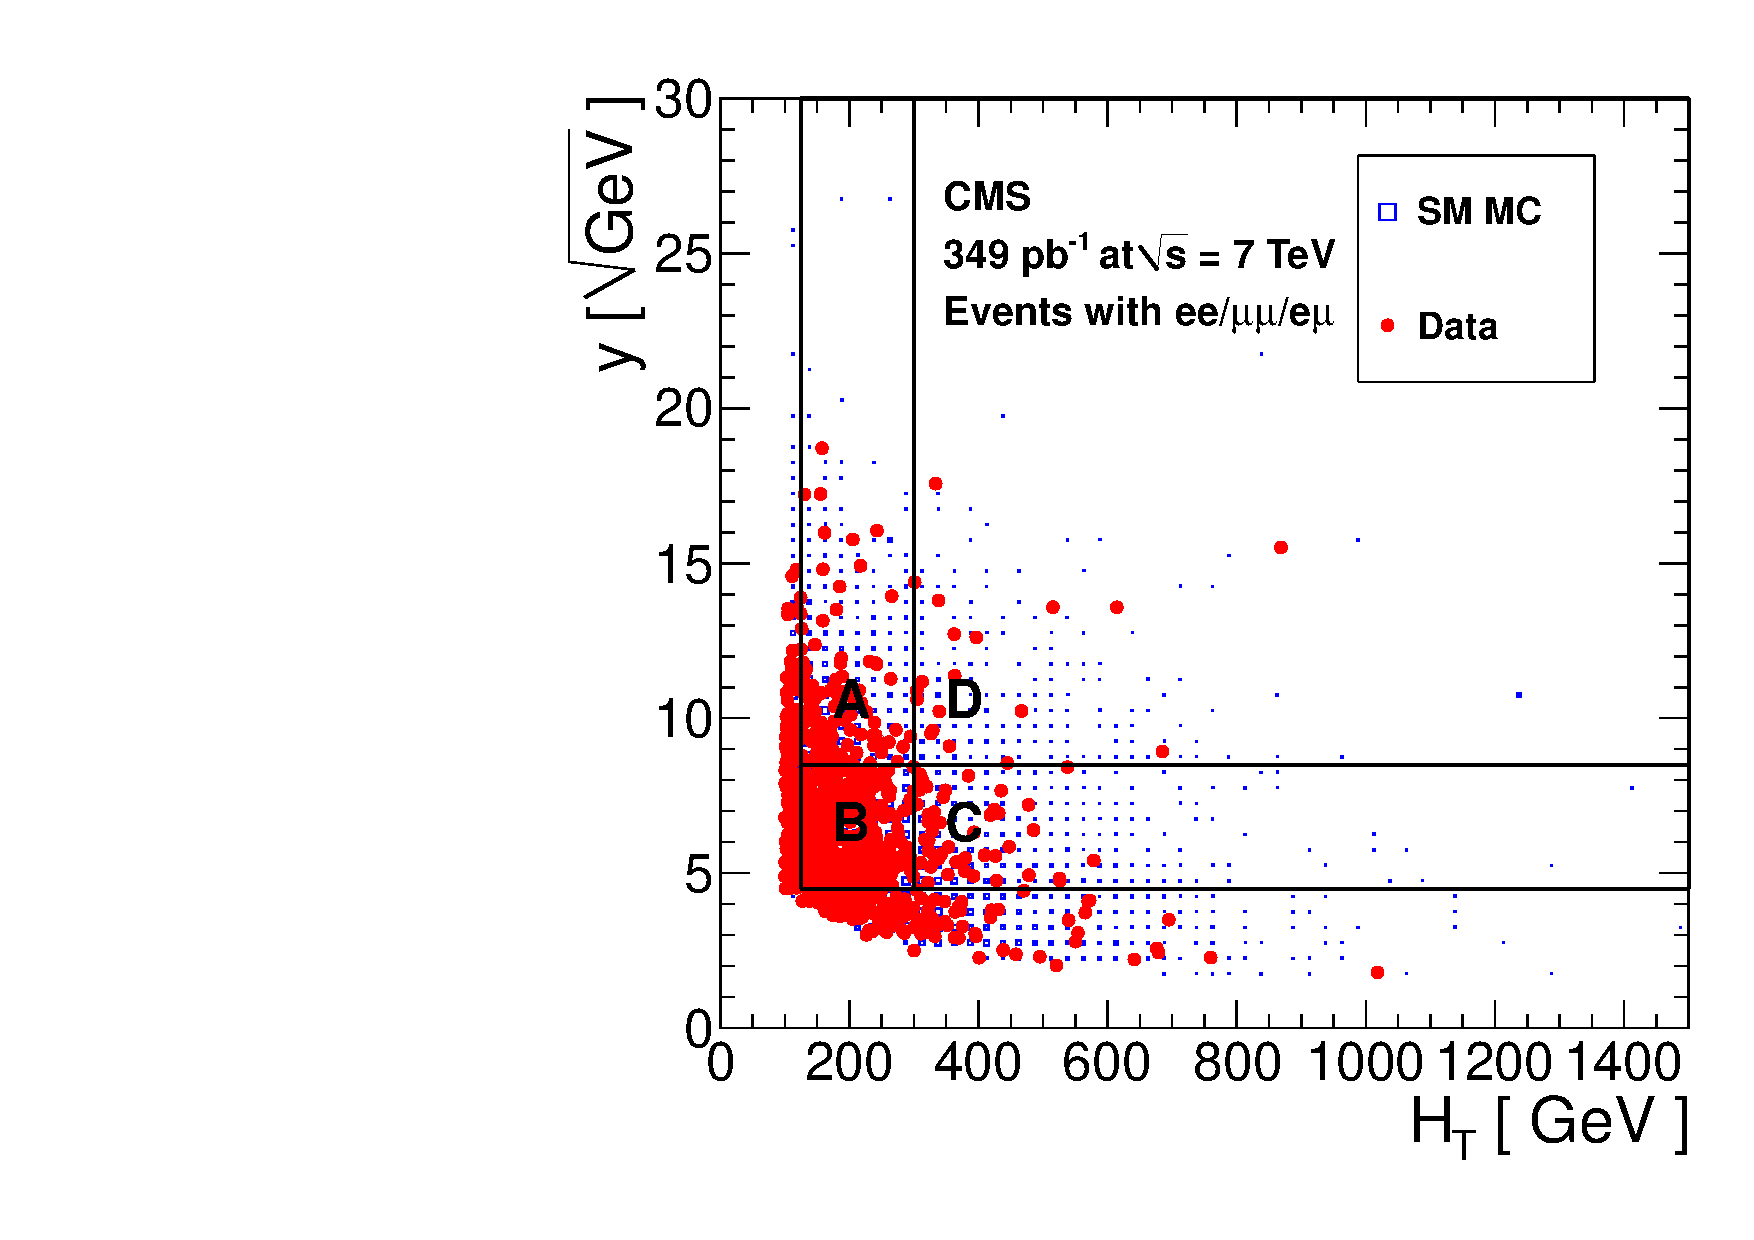
\includegraphics[width=0.6\linewidth]{plots/abcd_349pb.pdf}
\caption{\label{fig:abcdData1}\protect Distributions of $y$ 
vs. \Ht\ for SM Monte Carlo and data. The 2010 signal region boundaries are overlayed.}
\end{center}
\end{figure}

\begin{table}[hbt]
\begin{center}
\caption{\label{tab:datayield1} 
Data yields in the four
regions of Figure~\ref{fig:abcdData1} for the 2010 signal region, 
as well as the predicted yield in region D given
by $N_A \times N_C / N_B$.  The quoted uncertainty
on the prediction in data is statistical only, assuming Gaussian errors.
We also show the SM Monte Carlo expectations with statistical errors only.
}
\begin{tabular}{l||c|c|c|c||c}
\hline
           sample  &            $N_A$  &            $N_B$  &            $N_C$  &             $N_D$  &   $N_A \times N_C / N_B$ \\
\hline
            \ttll  & 63.9  $\pm$  2.0  &252.3  $\pm$  4.1  & 43.3  $\pm$  1.7  &  8.5  $\pm$  0.7  & 11.0  $\pm$  0.6        \\
           \tttau  & 18.5  $\pm$  1.1  & 55.9  $\pm$  1.9  & 10.3  $\pm$  0.8  &  3.4  $\pm$  0.5  &  3.4  $\pm$  0.4        \\
          \ttfake  &  1.0  $\pm$  0.3  &  6.6  $\pm$  0.7  &  1.1  $\pm$  0.3  &  0.4  $\pm$  0.2  &  0.2  $\pm$  0.1        \\
               DY  &  0.9  $\pm$  0.6  & 13.9  $\pm$  2.6  &  1.3  $\pm$  0.8  &  1.7  $\pm$  1.0  &  0.1  $\pm$  0.1        \\
              \WW  &  1.1  $\pm$  0.1  &  2.7  $\pm$  0.2  &  0.2  $\pm$  0.1  &  0.3  $\pm$  0.1  &  0.1  $\pm$  0.0        \\
              \WZ  &  0.1  $\pm$  0.0  &  0.6  $\pm$  0.0  &  0.1  $\pm$  0.0  &  0.0  $\pm$  0.0  &  0.0  $\pm$  0.0        \\
              \ZZ  &  0.0  $\pm$  0.0  &  0.2  $\pm$  0.0  &  0.0  $\pm$  0.0  &  0.0  $\pm$  0.0  &  0.0  $\pm$  0.0        \\
       single top  &  3.3  $\pm$  0.2  &  9.6  $\pm$  0.3  &  0.4  $\pm$  0.1  &  0.1  $\pm$  0.0  &  0.1  $\pm$  0.0        \\
           \wjets  &  1.0  $\pm$  1.0  &  2.2  $\pm$  1.1  &  0.0  $\pm$  0.0  &  0.0  $\pm$  0.0  &  0.0  $\pm$  0.0        \\
\hline
      Total SM MC  & 89.9  $\pm$  2.6  &344.0  $\pm$  5.3  & 56.6  $\pm$  2.1  & 14.5  $\pm$  1.4  & 14.8  $\pm$  0.7        \\
\hline
             data  &              110  &              381  &               44  &               19  & 12.7  $\pm$  2.4        \\
\hline
\end{tabular}
\end{center}
\end{table}


\begin{figure}[hbt]
\begin{center}
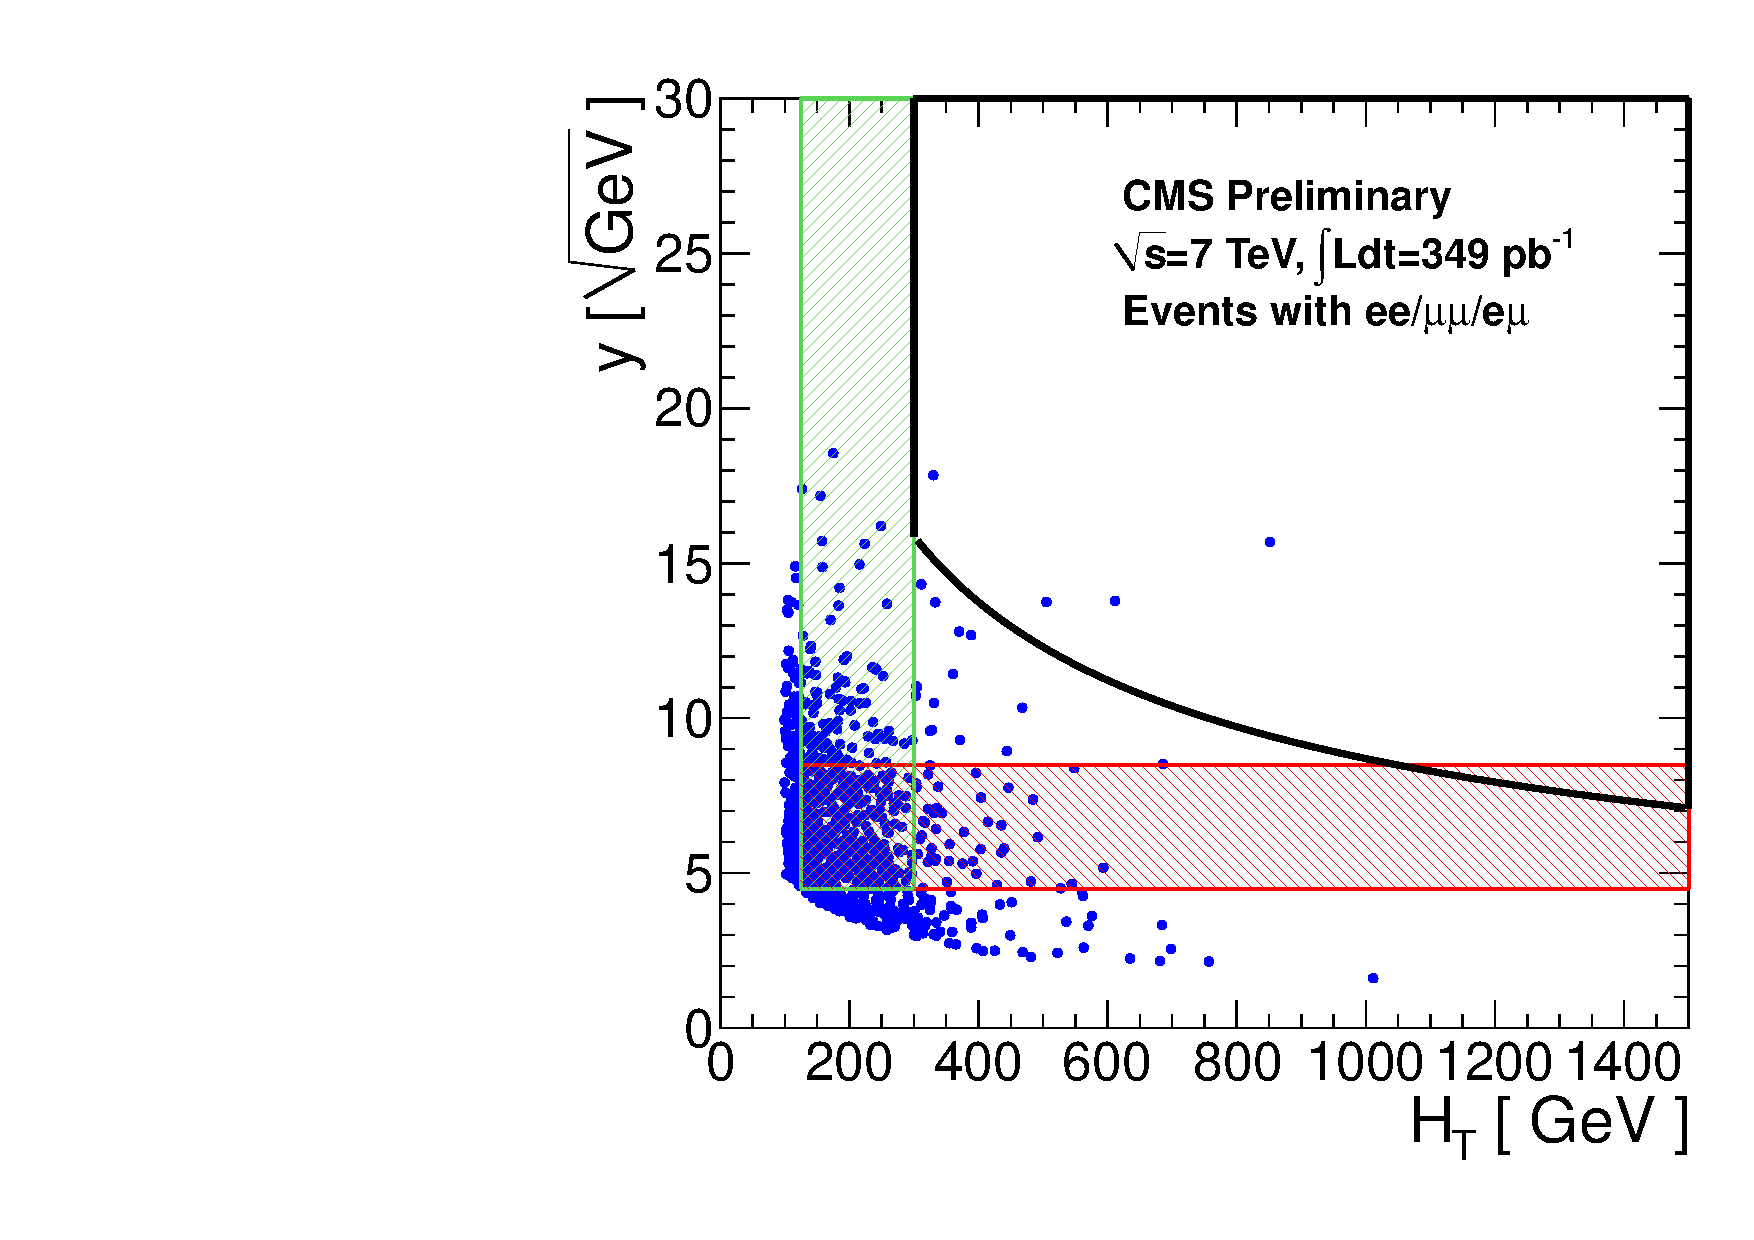
\includegraphics[width=0.48\linewidth]{plots/abcdprime_349pb_highmet.pdf}
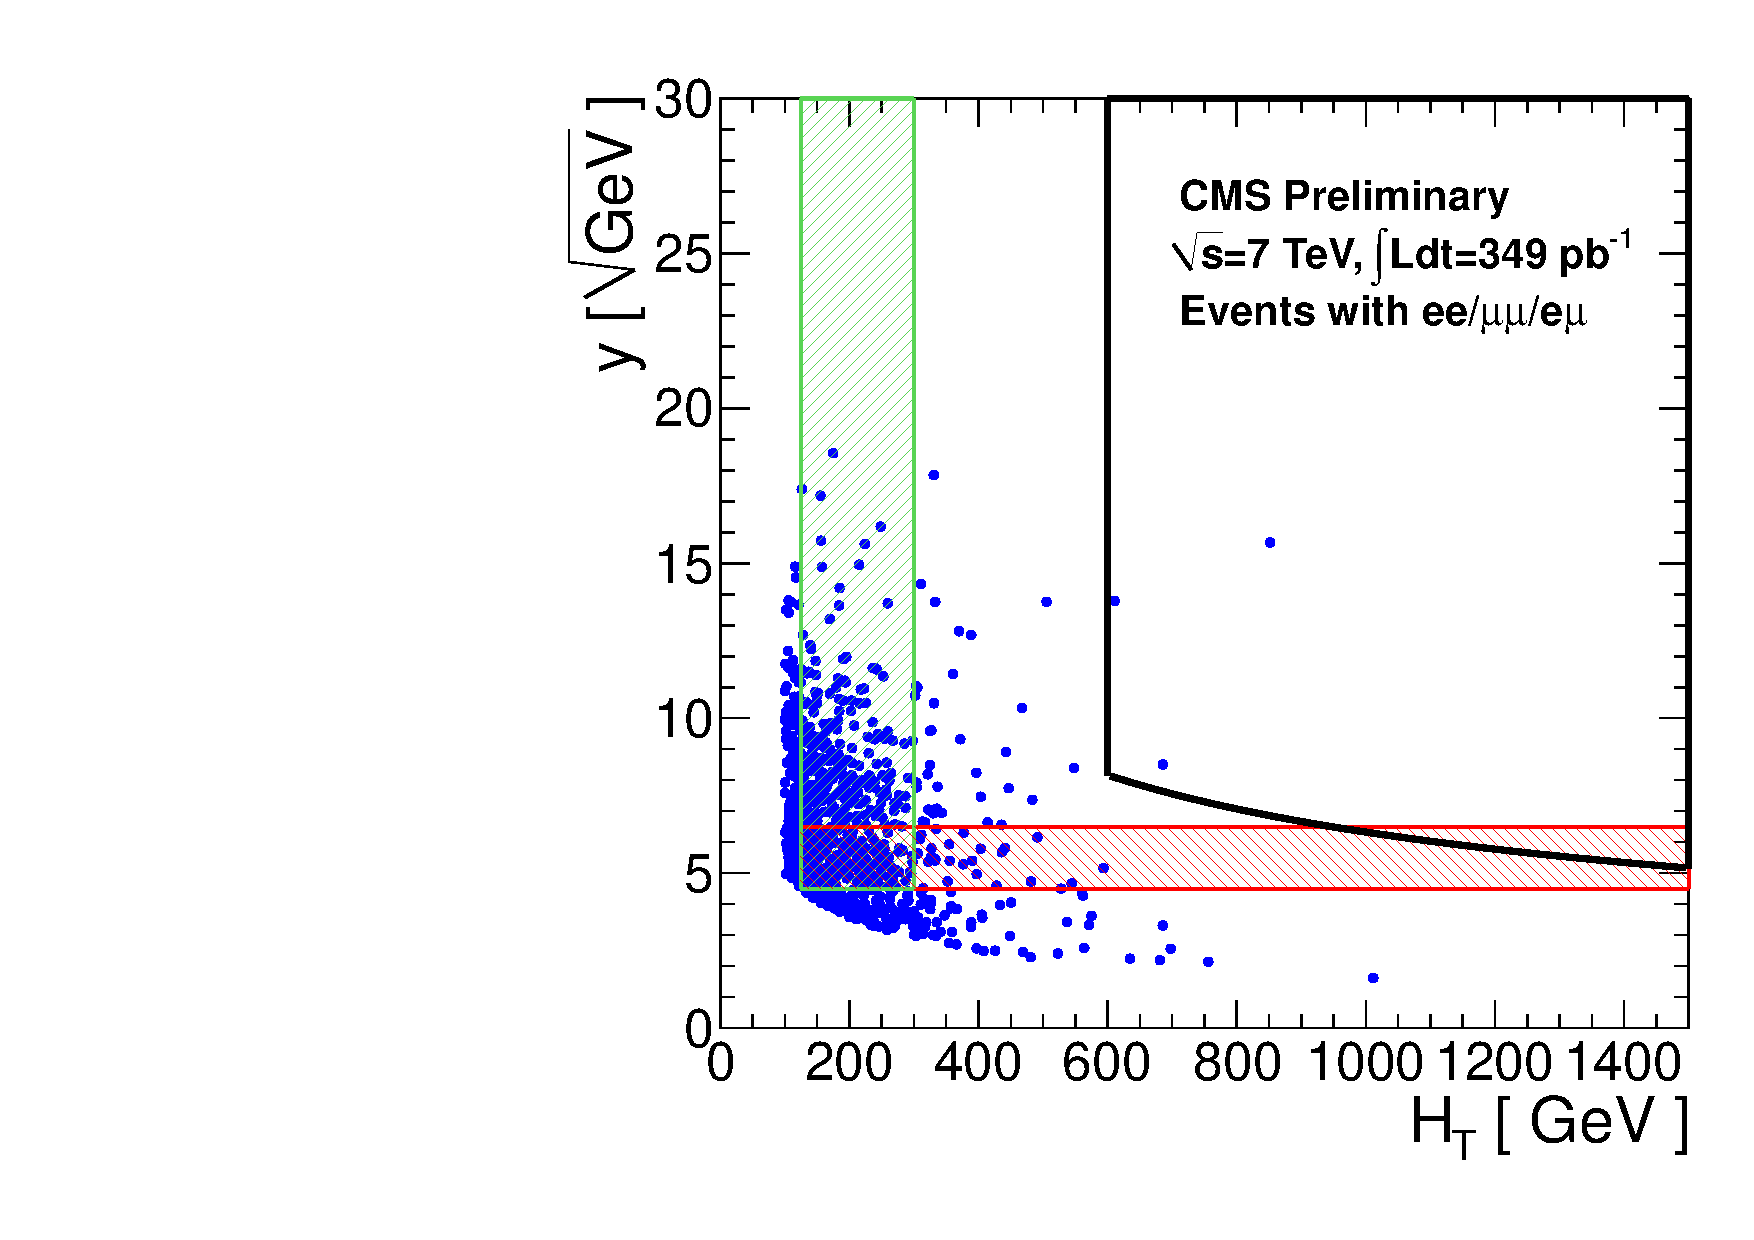
\includegraphics[width=0.48\linewidth]{plots/abcdprime_349pb_highht.pdf}
\caption{\label{fig:abcdprimedata}\protect 
Distributions of $y$ vs. \Ht\ in data. The signal regions \met\ $>$ 275 GeV, \Ht\ $>$ 300 GeV (left)
and \met\ $>$ 200 GeV, \Ht\ $>$ 600 GeV (right) are indicated with thick black lines. 
The $f(y)$ and $g(H_T)$ 
functions are measured using events in the green and red shaded areas, respectively.
}
\end{center}
\end{figure}

\subsection{Background estimate from the $P_T(\ell\ell)$ method}
\label{sec:victoryres}

We begin by extracting the value of the \met\ acceptance scaling factor $K$ from data,
for the \Ht\ control region 125--300 GeV and for the 2 signal regions \Ht\ $>$ 300 and
\Ht\ $>$ 600 GeV. The quantity $1/K$ is the efficiency for events passing preselection
and falling in the given \Ht\ range to pass the requirement \ptll\ $>$ 50 GeV.
The values of $K$ extracted from data and \ttbar\ MC are given in Table~\ref{tab:K}.
For all 3 \Ht\ regions, the value of $K$ extracted from data agrees with the 
\ttbar\ MC prediction, but for the \Ht\ $>$ 600 GeV region the statistical uncertainty
in $K$ from data is $\sim$100\%. Therefore we use the value of $K$ extracted from
data for the control region 125--300 GeV and for the signal regions \Ht\ $>$ 300;
for the \Ht\ $>$ 600 GeV region we use $K$ from \ttbar\ MC.


\begin{table}[hbt]
\begin{center}
\caption{\label{tab:K} 
Summary of the \met\ acceptance scaling factor $K$, extracted from data and \ttbar\ MC.
}
\begin{tabular}{lccccc}
\hline
region                                    &  data              &   \ttbar\ MC      \\
\hline
control region: 125 $<$ \Ht\ $<$ 300 GeV  &  1.68 $\pm$ 0.14   &   1.67 $\pm$ 0.03 \\
signal region: \Ht\ $>$ 300 GeV           &  1.45 $\pm$ 0.29   &   1.50 $\pm$ 0.06 \\
signal region: \Ht\ $>$ 600 GeV           &  1.12 $\pm$ 1.19   &   1.32 $\pm$ 0.20 \\
\hline
\end{tabular}
\end{center}
\end{table}



\begin{table}[hbt]
\begin{center}
\caption{\label{tab:victory} 
Summary of results of the dilepton $p_{T}$ template method applied to the 3 signal regions.
The quantities indicated in the table are discussed in the text.
The quoted statistical uncertainty in the prediction $N_P$ is due to
that of $N(D')$, the quoted systematic uncertainty includes that of $N(DY)$, $K$, and $K_C$.
%{\bf K and KC taken from MC, do we want to take K and/or KC from data? }
%{\bf Need to add jet/met uncertainty here}
%{\color{red} \bf CURRENTLY USING 30\% UNCERTAINTY ON K_C IN 2010 REGION, WHICH IS WHAT WE HAD LAST YEAR (NEED TO REPEAT JET/MET UNCERTAINTIES?).}
%{\color{red} \bf FOR HIGH Y/HIGH HT REGION, TAKING SYST UNCERTAINTY ON KC FROM MC STATS, WHICH IS PROBABLY DOMINANT}
}
\begin{tabular}{lccccc}
\hline
Signal Region               &  $N(D')$   &   $N(DY)$         &          $K$   &   $K_C$        & $N_P$                                   \\ 
\hline
2010 signal region (UPDATE) &       9    &   0.8 $\pm$ 0.4   & 1.5 $\pm$ 0.3  & 1.4 $\pm$ 0.4  & 16.7 $\pm$ 6.1 (stat) $\pm$ 5.9 (syst)  \\
high \met\ signal region    &       3    &   0.5 $\pm$ 0.3   & 1.5 $\pm$ 0.3  & 1.5 $\pm$ 0.5  & 5.4 $\pm$ 3.8 (stat) $\pm$ 2.2 (syst)   \\
high \Ht\ signal region     &       1    &   0.0 $\pm$ 0.0   & 1.3 $\pm$ 0.2  & 1.3 $\pm$ 0.4  & 1.7 $\pm$ 1.7 (stat) $\pm$ 0.6 (syst)   \\
\hline
\end{tabular}
\end{center}
\end{table}

For each signal region D, we count the number of events falling in the region D', which is defined
using the same requirements as D but switching the $y$ requirement to a $\ptll/\sqrt{H_T}$ requirement (2010 signal region)
or switching the \met\ requirement to a \ptll\ requirement (high \met\ and high \Ht\ signal regions).
We subtract off the expected DY contribution using the data-driven $R_{out/in}$ technique, using $R_{out/in} = 0.13 \pm 0.07$.
%{\color{red} \bf add plot justifying this value}. 
We then scale this yield by 2 corrections factors:
$K$, the \met\ acceptance correction factor, and $K_C$, the correction factor determined in Sec.~\ref{sec:datadriven}.
Our final prediction $N_P$ is given by:

\begin{center}
$ N_P = (N(D')-N(DY)) \times K \times K_C$,
\end{center}

as summarized in Table~\ref{tab:victory}, and displayed in Figs.~\ref{fig:vic1}-\ref{fig:vic3}.
We also perform the \ptll\ method in the \Ht\ sideband region 125--300~GeV, as a validation of the technique in a high statistics
sample which is expected to be dominated by background. The results are summarized in Table~\ref{tab:victorycontrol}
and displayed in Fig.~\ref{fig:victorycontrol}.
The prediction is extractedd for the requirement $y > 8.5$~GeV$^{1/2}$ corresponding to the 2010 signal region, as well as
for \met\ $>$ 200 GeV corresponding to the high \Ht\ signal region. In both cases, we observe good agreement between
the predicted and observed yields. 


\begin{table}[hbt]
\begin{center}
\caption{\label{tab:victorycontrol} 
Summary of results of the dilepton $p_{T}$ template method applied to the \Ht\ sideband control region 125--300 GeV.
The quantities indicated in the table are discussed in the text.
The quoted statistical uncertainty in the prediction $N_P$ is due to
that of $N(D')$, the quoted systematic uncertainty includes that of $N(DY)$ and $K_C$.
The predictions are compare with the observed yield $N_O$.
}
\begin{tabular}{lcccccc}
\hline
Control Region                                   &  $N(D')$   &   $N(DY)$        &  $K$          &   $K_C$          & $N_P$                                     & $N_O$ \\ 
\hline                                           
125 $<$ \Ht\ $<$ 300~GeV, $y >$ 8.5~GeV$^{1/2}$  &     54      &  2.6 $\pm$ 1.2   & 1.7 $\pm$ 0.1 & 1.4 $\pm$ 0.1    & 120.9 $\pm$ 17.3 (stat) $\pm$ 13.6 (syst) & 110   \\
125 $<$ \Ht\ $<$ 300~GeV, \met\ $>$ 200 GeV     &      4      &  1.0 $\pm$ 0.5   & 1.7 $\pm$ 0.1 & 1.3 $\pm$ 0.2    &   6.5 $\pm$  4.4 (stat) $\pm$  1.6 (syst) &   6   \\
\hline
\end{tabular}
\end{center}
\end{table}



\begin{figure}[hbt]
\begin{center}
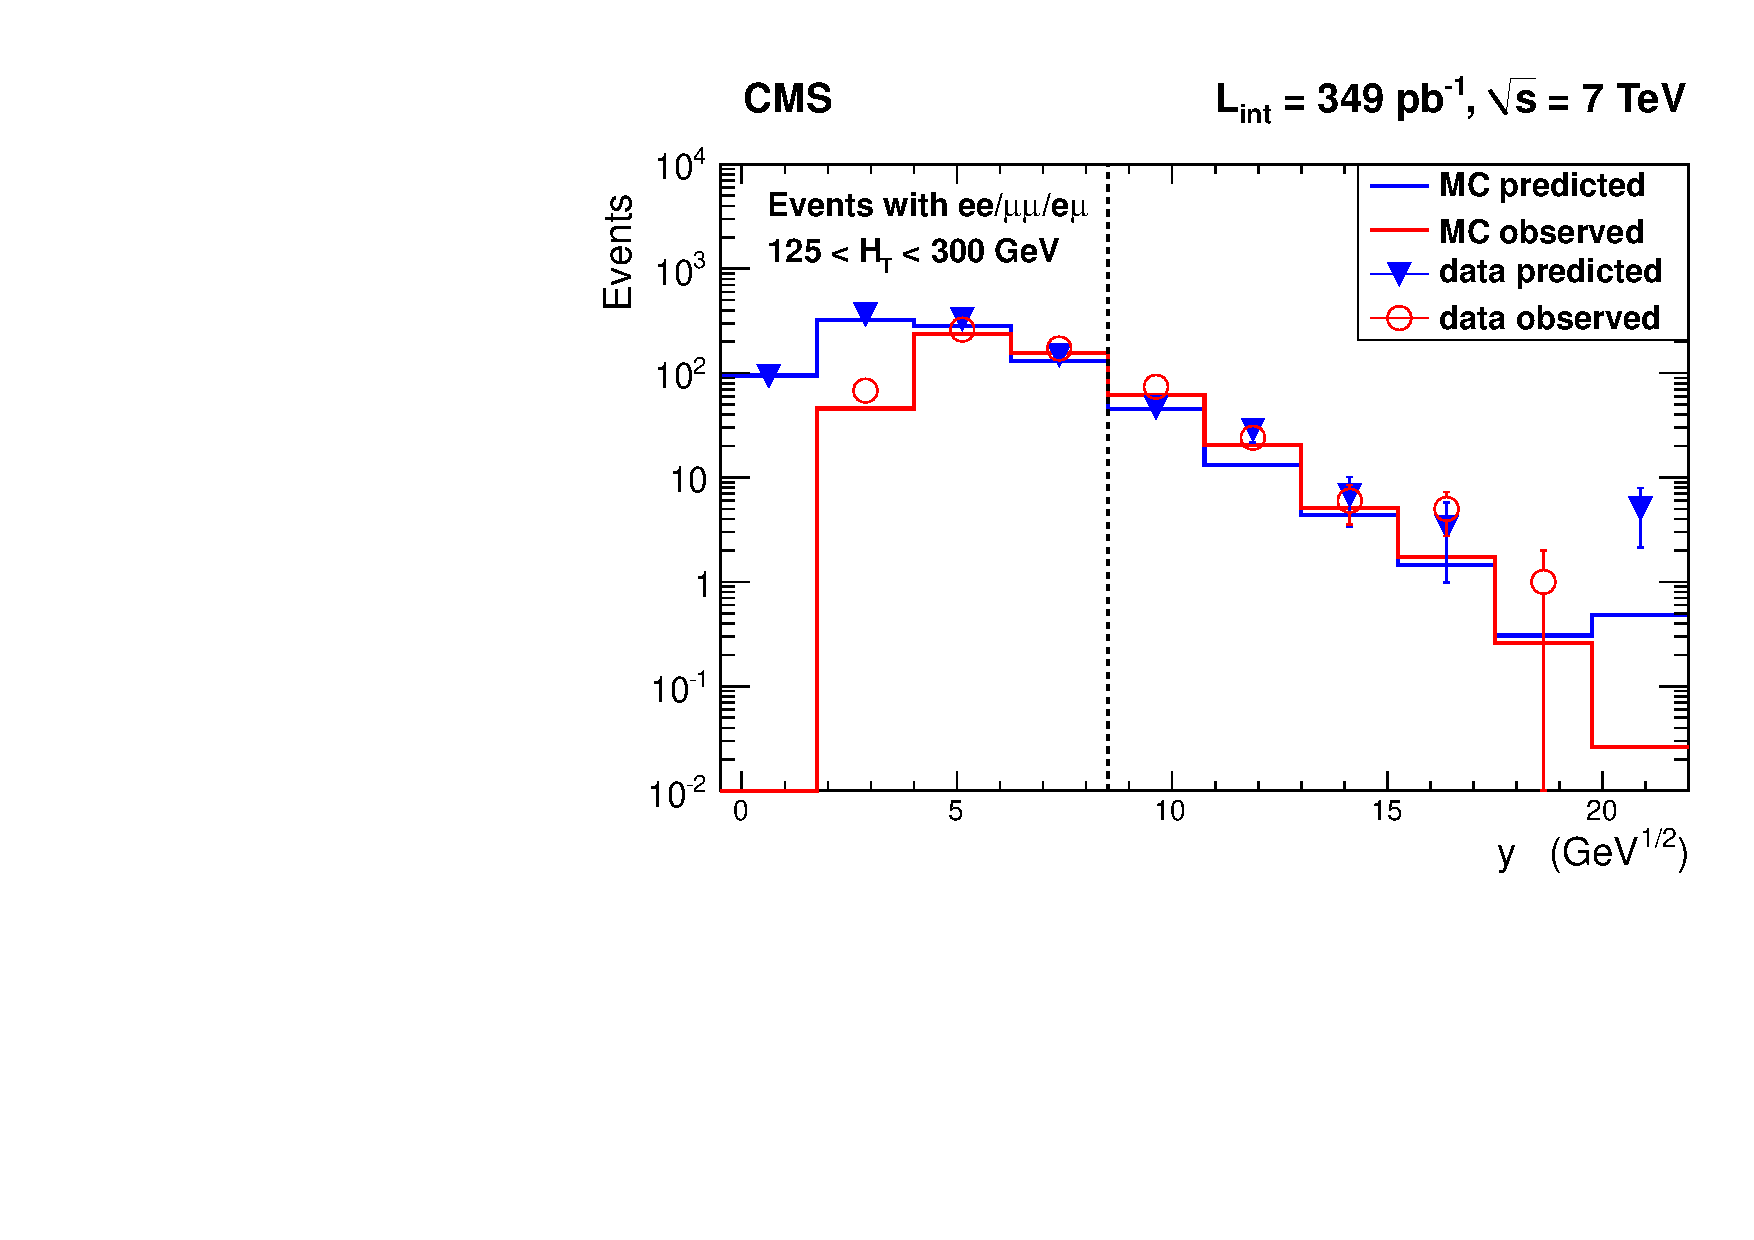
\includegraphics[width=0.48\linewidth]{plots/victory_y_control_349pb.pdf}
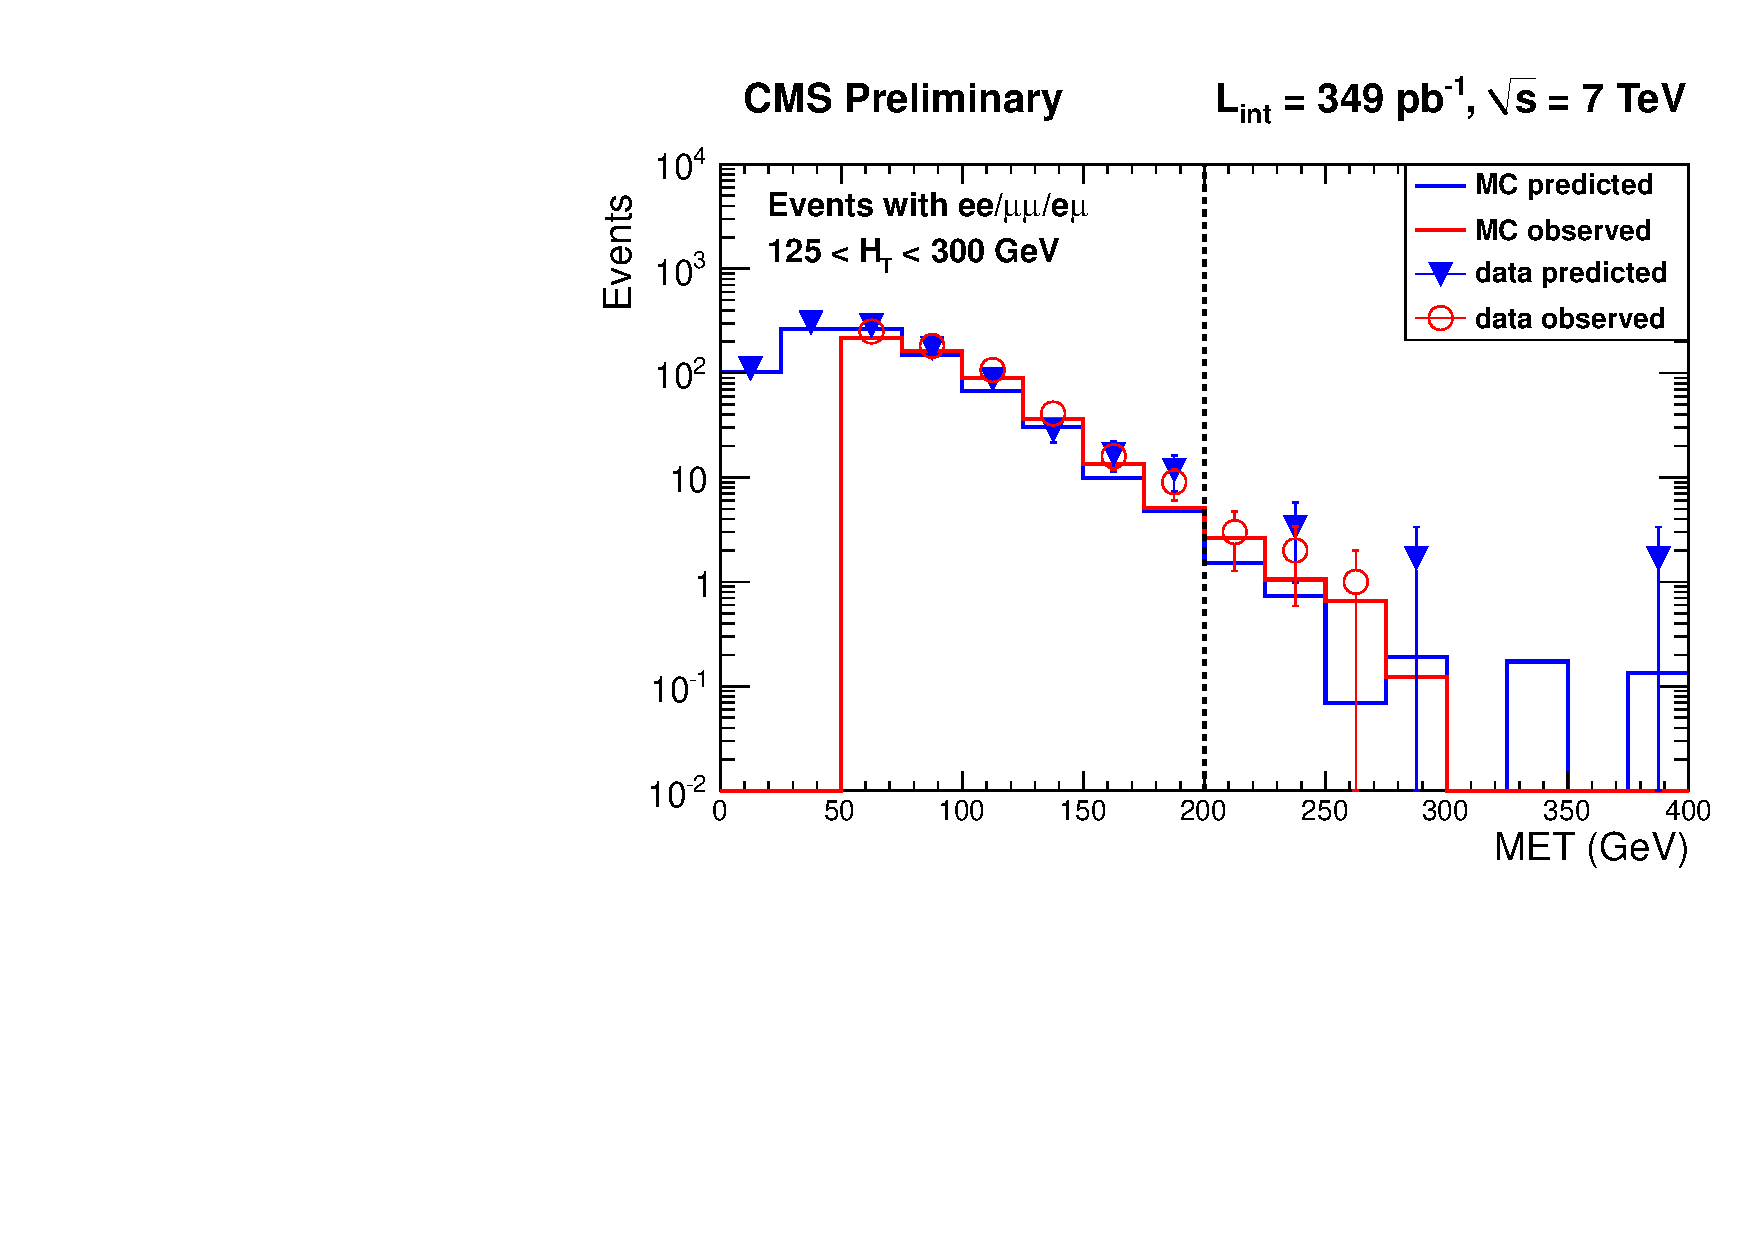
\includegraphics[width=0.48\linewidth]{plots/victory_met200_control_349pb.pdf}
\caption{\label{fig:victorycontrol}\protect 
Results of the \ptll\ method in the \Ht\ sideband region 125-300 GeV.
Left:  distributions of $\ptll/\sqrt{H_T}$ (predicted) and $y$ (observed) for 
SM MC and data. The vertical dashed lines indicate the requirement $y > 8.5$~GeV$^{1/2}$),
corresponding to the 2010 signal region.
Right: distributions of \ptll\ (predicted) and \met\ (observed) for 
SM MC and data. The vertical dashed lines indicate the requirement \met\ $>$ 200 GeV,
corresponding to the high \Ht\ signal region.
}
\end{center}
\end{figure}


\begin{figure}[tbh]
\begin{center}
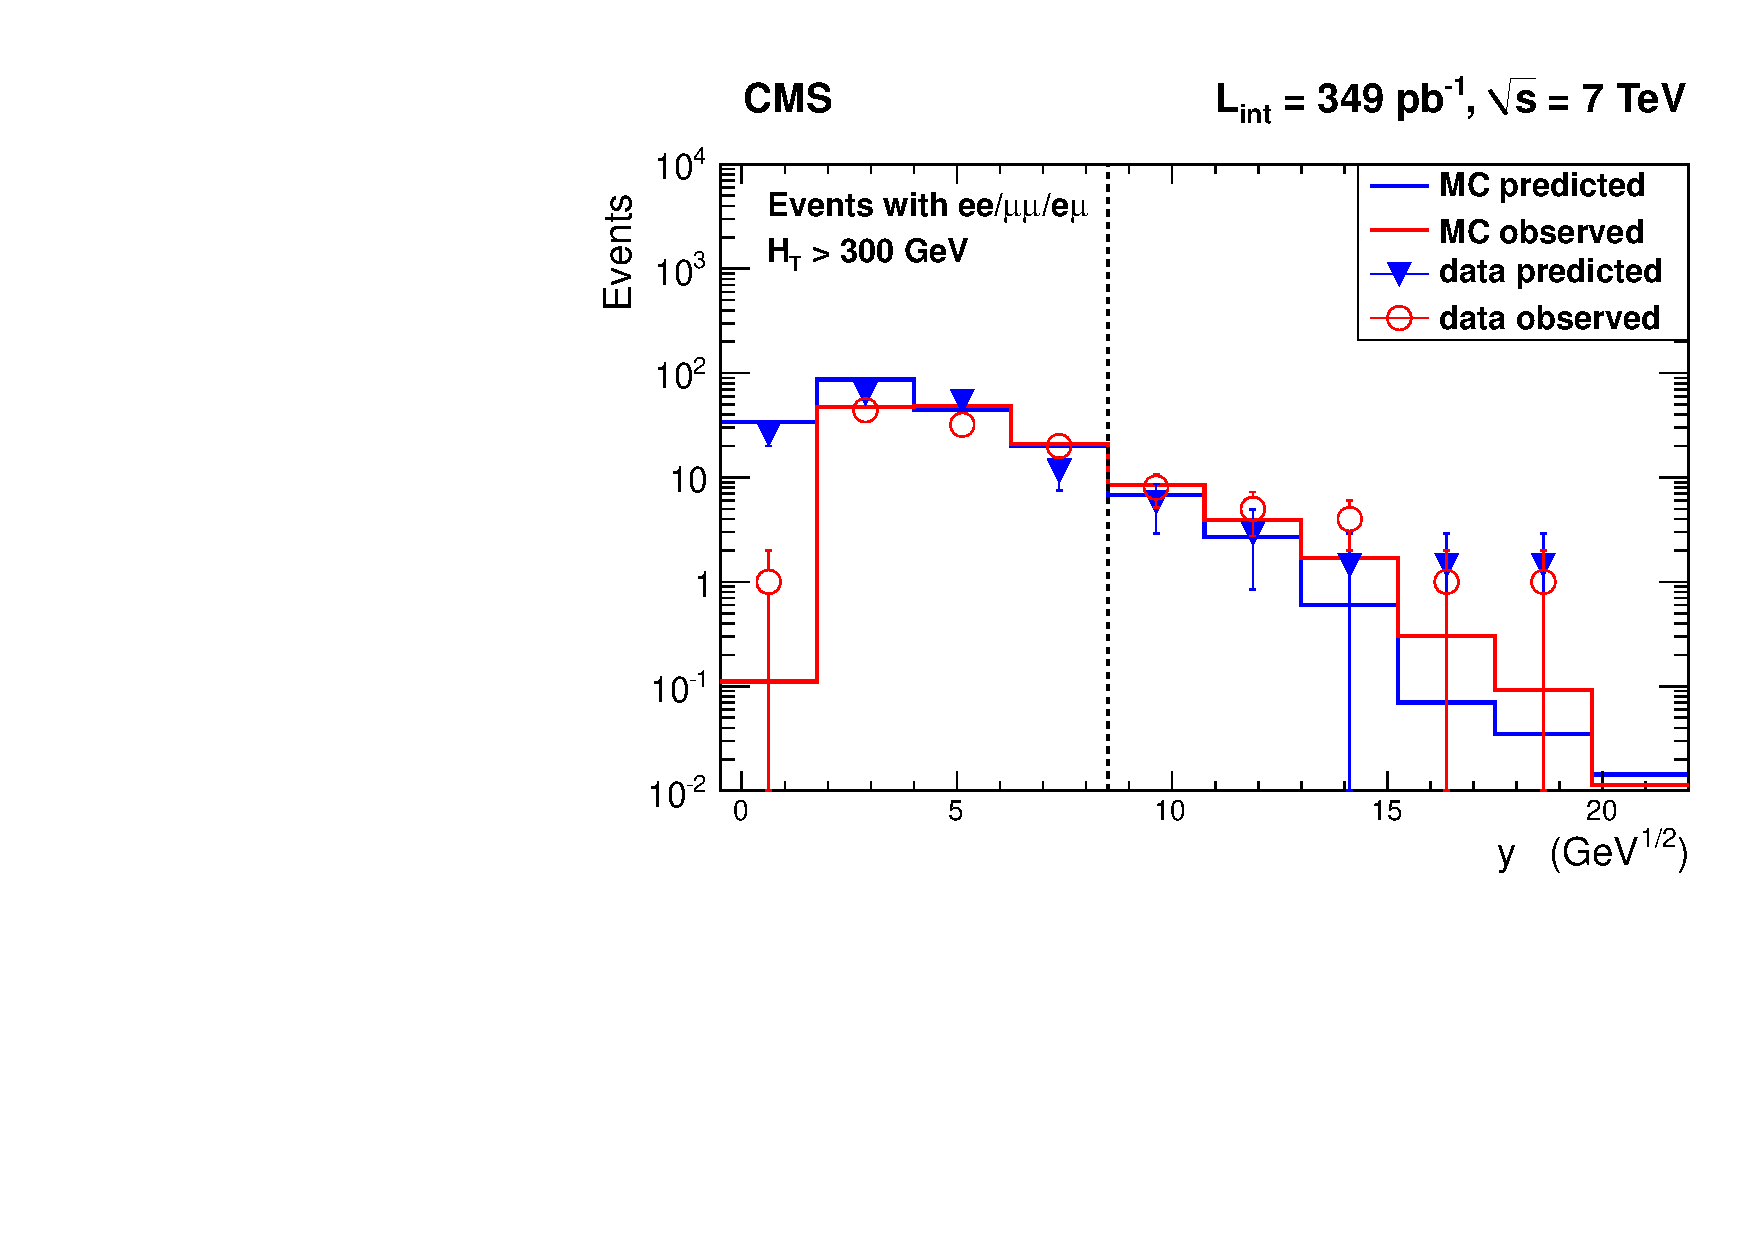
\includegraphics[width=0.6\linewidth]{plots/victory_y_ht300_349pb.pdf}
\caption{\label{fig:vic1}\protect 
Distributions of $\ptll/\sqrt{H_T}$ (predicted) and $y$ (observed) for 
SM MC and data, for the \Ht $>$ 300 GeV. 
The vertical dashed lines indicate the requirement $y > 8.5$~GeV$^{1/2}$ corresponding to the 2010 signal region.
}
\end{center}
\end{figure}

\begin{figure}[tbh]
\begin{center}
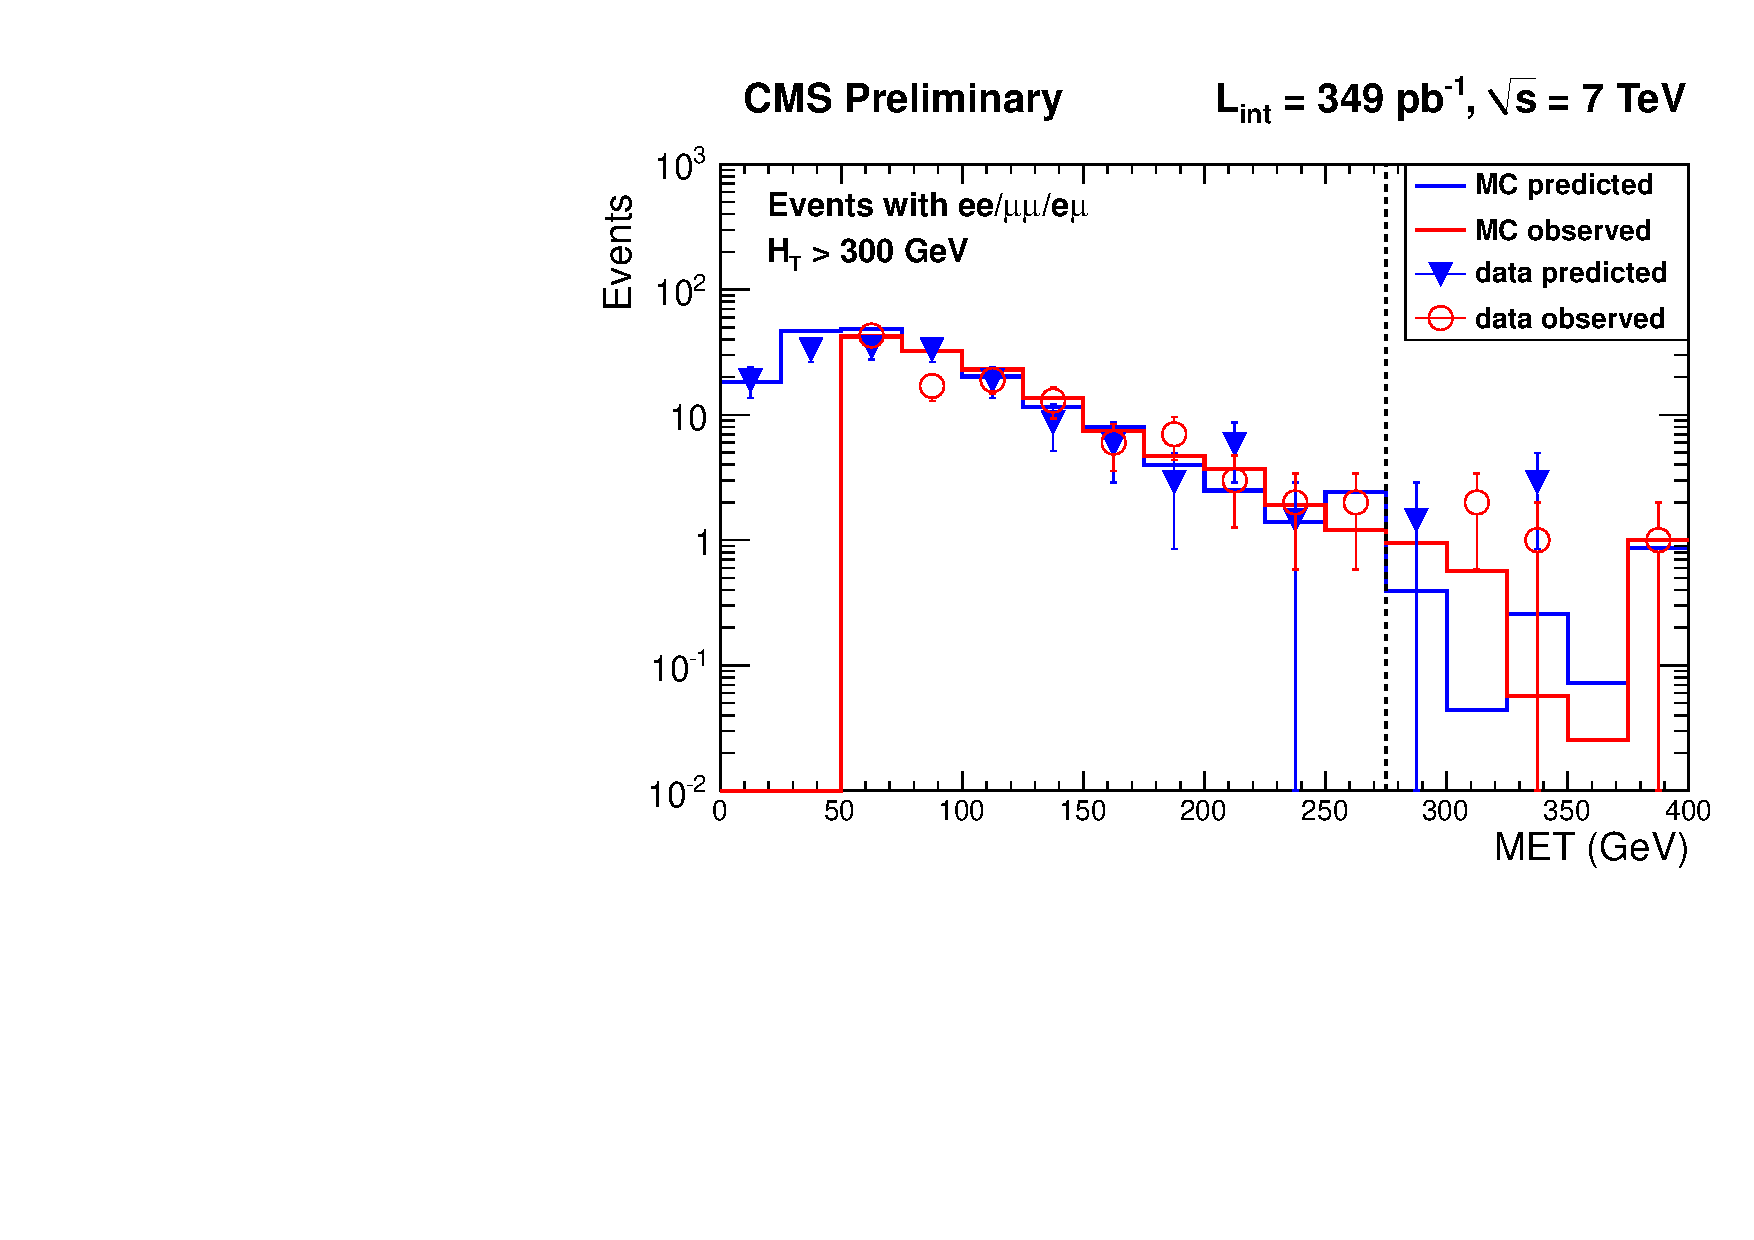
\includegraphics[width=0.6\linewidth]{plots/victory_met275_ht300_349pb.pdf}
\caption{\label{fig:v2}\protect 
Distributions of \ptll\ (predicted) and \met\ (observed) for 
SM MC and data, for the region \Ht $>$ 300 GeV. 
The vertical dashed lines indicate the requirement \met\ $>$ 275 GeV, corresponding to the high \met\ signal region.
}
\end{center}
\end{figure}

\begin{figure}[tbh]
\begin{center}
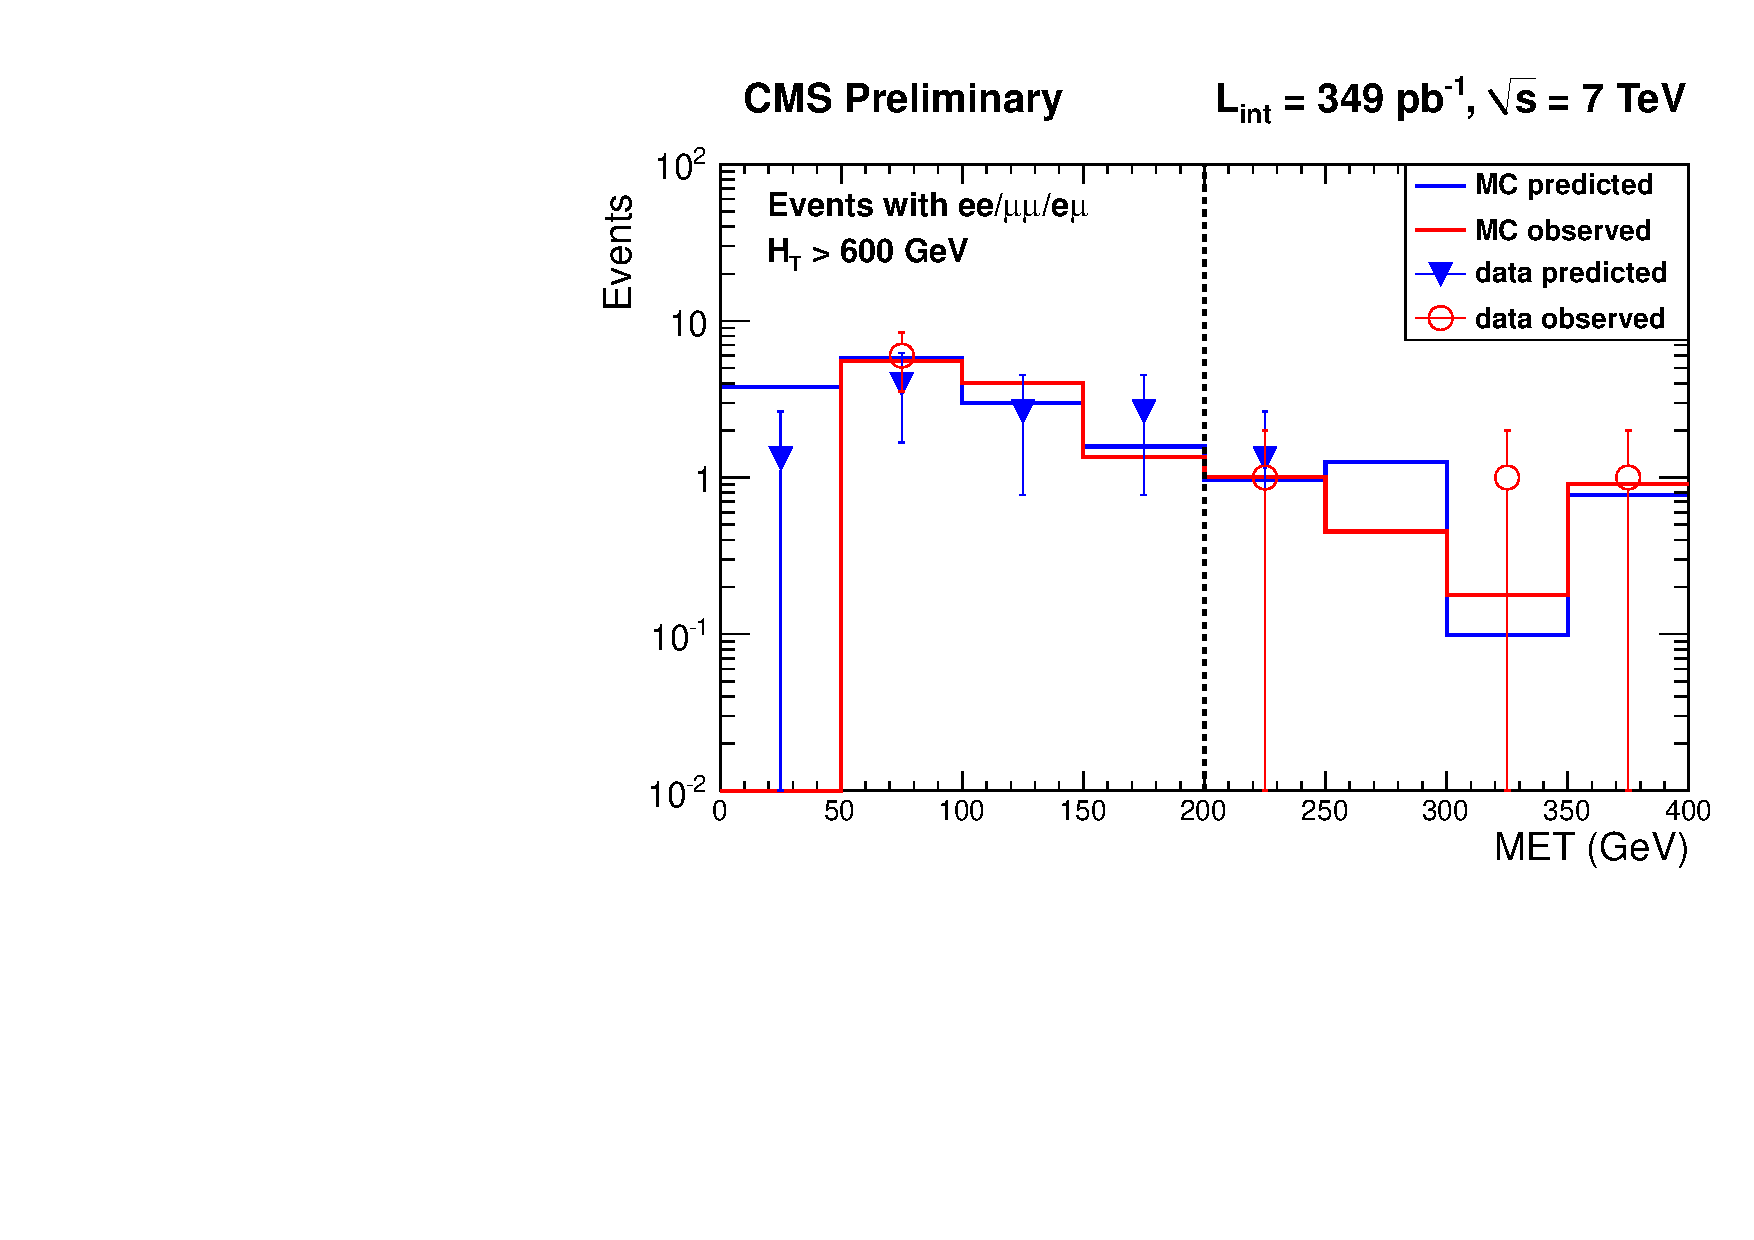
\includegraphics[width=0.6\linewidth]{plots/victory_met200_ht600_349pb.pdf}
\caption{\label{fig:vic3}\protect 
Distributions of \ptll\ (predicted) and \met\ (observed) for 
SM MC and data, for the region \Ht $>$ 600 GeV. 
The vertical dashed lines indicate the requirement \met\ $>$ 200 GeV, corresponding to the high \Ht\ signal region.
}
\end{center}
\end{figure}

\subsection{Background estimate from OF subtraction}
\label{sec:ofres}

The results of the OF subtraction technique applied to the high \pt\ dilepton trigger sample are summarized in Table~\ref{tab:ofres}. 
We evaluate the quantity $\Delta = R_{\mu e}N(ee) + \frac{1}{R_{\mu e}}N(\mu\mu) - N(e\mu)$ with $R_{\mu e} = 1.12 \pm 0.05$
extracted from the ratio of $Z \to \mu^+\mu^-$ vs. $Z \to e^+e^-$ events in data.
We perform the OF subtraction first in the preselection region, and find $\Delta$ consistent with 0, as expected.
We then perform the OF subtraction in all 3 signal regions, and do not observe any excess of same-flavor vs. opposite-flavor events.

\begin{table}[hbt]
\begin{center}
\caption{\label{tab:ofres} Summary of results for the OF subtraction technique. 
The quantity $\Delta = R_{\mu e}N(ee) + \frac{1}{R_{\mu e}}N(\mu\mu) - N(e\mu)$ is quoted with $R_{\mu e} = 1.12 \pm 0.05$.
The quoted systematic uncertainty corresponds to that of $R_{\mu e}$. The $e\mu$ yields differ from those previously
quoted because the $Z$ mass veto is included here.
}
\begin{tabular}{l|ccc|c}
\hline
region                   &  $N(ee)$ & $N(\mu\mu)$ & $N(e\mu)$  &  $\Delta$   \\ 
\hline
preselection region      &      193 &         201 &      394   &    2.0 $\pm$ 28 (stat) $\pm$ 1.8 (syst) \\    
2010 signal region       &        4 &           4 &        9   &   -0.9 $\pm$ 4.2 (stat) $\pm$ 0.1 (syst)  \\
high \met\ signal region &        2 &           0 &        1   &    1.3 $\pm$ 1.9 (stat) $\pm$ 0.1 (syst)  \\
high \Ht\ signal region  &        1 &           0 &        1   &    0.1 $\pm$ 1.5 (stat) $\pm$ 0.0 (syst)  \\
\hline
\end{tabular}
\end{center}
\end{table}

For the dilepton-\Ht\ trigger sample, we observe only 1 event in the 2010 signal region, consistent with MC expectations,
and no events in either the high $y$ or high \Ht\ signal regions. In the case of an excess of events at low lepton \pt,
we will perform the OF subtraction technique of Sec.~\ref{sec:oflowpt}.

% \clearpage
\subsection{Summary of results}

\begin{table}[hbt]
\begin{center}
\caption{\label{tab:results} 
Summary of the observed and predicted yields in the 3 signal regions. MC errors are statistical only. The systematic uncertainty on the ABCD
and \ptll\ method is from the scaling factors from MC closure only. 
%{\bf need to put additional uncertainties, for example jet/met scale.}
For the OF subtraction, the quantity $\Delta = R_{\mu e}N(ee) + \frac{1}{R_{\mu e}}N(\mu\mu) - N(e\mu)$ is quoted; the systematic uncertainty
here is from the ratio of muon to electron selection efficiencies.
}
\begin{tabular}{l|c|c|c}
\hline
                                       &  2010 signal region                       &   high \met\ signal region             &  high \Ht\ signal region              \\ 
\hline
Observed yield                         &         19                                &                        4               &                        3              \\
\hline
MC prediction                          &    14.5 $\pm$ 1.4                         &            2.6 $\pm$ 0.8               &            2.5 $\pm$ 0.8              \\
ABCD prediction                        &    12.7 $\pm$ 2.4 (stat) $\pm$ 2.5 (syst) &                                        &                                       \\
ABCD' prediction                       &    12.8 $\pm$ 2.9 (stat) $\pm$ 2.6 (syst) & 1.2 $\pm$ 0.4 (stat) $\pm$ 0.5 (syst)  & 0.0 $\pm$ 0.6 (stat) $\pm$ 0.3 (syst) \\
\ptll\ prediction                      &    16.7 $\pm$ 6.1 (stat) $\pm$ 5.9 (syst) & 5.4 $\pm$ 3.8 (stat) $\pm$ 2.2 (syst)  & 1.7 $\pm$ 1.7 (stat) $\pm$ 0.6 (syst) \\
\hline
OF subtraction ($\Delta$)              &    -0.9 $\pm$ 4.2 (stat) $\pm$ 0.1 (syst) & 1.3 $\pm$ 1.9 (stat) $\pm$ 0.1 (syst)  & 0.1 $\pm$ 1.5 (stat) $\pm$ 0.0 (syst) \\
\hline
\end{tabular}
\end{center}
\end{table}

A summary of our results is presented in Table~\ref{tab:results}. In all 3 signal regions, we observe reasonable agreement
between the observed yields and the predictions from MC and data-driven background estimates. We therefore do not observe
evidence for an excess of events above SM expectations. After assessing systematic uncertainties in Sec.~\ref{sec:systematics},
we proceed to set upper limits on the non-SM contributions to the signal regions in Sec.~\ref{sec:limits}.

%\section{Systematics Uncertainties in the Background Prediction}
\label{sec:systematics}

The methodology for determining the systematics on the background
predictions has not changed with respect to the nominal analysis.
Because the template method has not changed, the same 
systematic uncertainty is assessed on this prediction (32\%).
The 50\% uncertainty on the WZ and ZZ background is also unchanged.
The systematic uncertainty in the OF background prediction based on 
e$\mu$ events has changed, due to the different composition of this
sample after vetoing events containing b-tagged jets.

As in the nominal analysis, we do not require the e$\mu$ events
to satisfy the dilepton mass requirement and apply a scaling factor K,
extracted from MC, to account for the fraction of e$\mu$ events
which satisfy the dilepton mass requirement. This procedure is used
in order to improve the statistical precision of the OF background estimate.

For the selection used in the nominal analysis, 
the e$\mu$ sample is completely dominated by $t\bar{t}$
events, and we observe that K is statistically consistent with constant with
respect to the \MET\ requirement. However, in this analysis, the $t\bar{t}$
background is strongly suppressed by the b-veto, and hence the non-$t\bar{t}$
backgrounds (specifically, $Z\to\tau\tau$ and VV) become more relevant. 
At low \MET, the $Z\to\tau\tau$ background is pronounced, while $t\bar{t}$
and VV dominate at high \MET\ (see App.~\ref{app:kinemu}).
Therefore, the sample composition changes
as the \MET\ requirement is varied, and as a result K depends
on the \MET\ requirement. 

We thus measure K in MC separately for each
\MET\ requirement, as displayed in Fig.~\ref{fig:kvmet} (left).
%The systematic uncertainty on K is determined separately for each \MET\
%requirement by comparing the relative difference in K in data vs. MC.
The values of K used are the MC predictions 
%and the total systematic uncertainty on the OF prediction 
%as shown in 
(Table \ref{fig:kvmettable}).
The contribution to the total OF prediction systematic uncertainty 
from K is assessed from the ratio of K in data and MC,
shown in Fig.~\ref{fig:kvmet} (right).
The ratio is consistent with unity to roughly 17\%, 
so we take this value as the systematic from K.
17\% added in quadrature with 7\% from 
the electron to muon efficieny ratio 
(as assessed in the inclusive analysis)
yields a total systematic of $\sim$18\% 
which we round up to 20\%.
For \MET\ $>$ 150, there are no OF events in data inside the Z mass window
so we take a systematic based on the statistical uncertainty
of the MC prediction for K. 
This value is 25\% for \MET\ $>$ 150 GeV and 60\% for \MET\ $>$ 200 GeV.
%Although we cannot check the value of K in data for \MET\ $>$ 150
%because we find no OF events inside the Z mass window for this \MET\ 
%cut, the overall OF yields with no dilepton mass requirement 
%agree to roughly 20\% (9 data vs 7.0 $\pm$ 1.1 MC).


%Below Old

%In reevaluating the systematics on the OF prediction, however,
%we observed a different behavior of K as a function of \MET\ 
%as was seen in the inclusive analysis. 

%Recall that K is the ratio of the number of \emu\ events
%inside the Z window to the total number of \emu\ events.
%In the inclusive analysis, it is taken from \ttbar\ MC
%and used to scale the inclusive \emu\ yield in data.
%The yield scaled by K is then corrected for 
%the $e$ vs $\mu$ efficiency difference to obtain the 
%final OF prediction.

%Based on the plot in figure \ref{fig:kvmet}, 
%we choose to use a different
%K for each \MET\ cut and assess a systematic uncertainty
%on the OF prediction based on the difference between 
%K in data and MC. 
%The variation of K as a function of \MET\ is caused 
%by a change in sample composition with increasing \MET.
%At \MET\ $<$ 60 GeV, the contribution of Z plus jets is
%not negligible (as it was in the inclusive analysis)
%because of the b veto. (See appendix \ref{app:kinemu}.)
%At higher \MET, \ttbar\ and diboson backgrounds dominate.




\begin{figure}[hbt]
  \begin{center}
	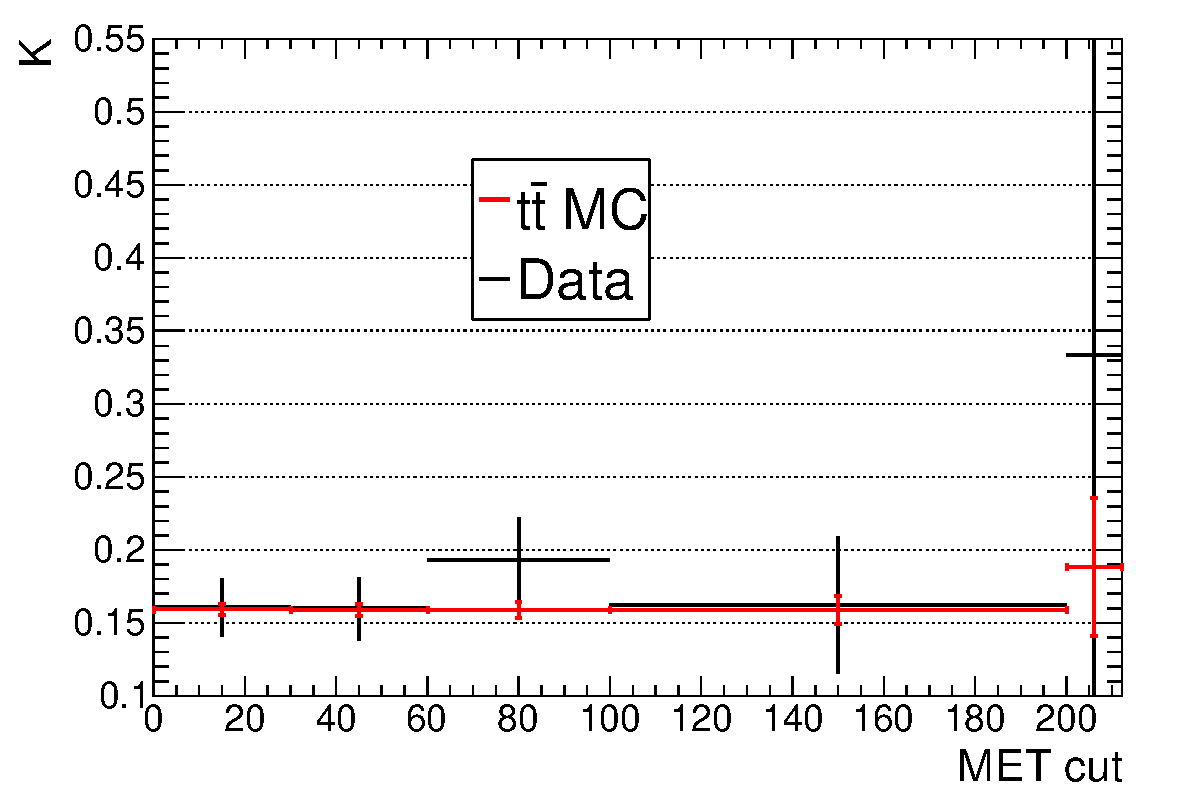
\includegraphics[width=0.48\linewidth]{plots/kvmet_data_ttbm.pdf}
	\includegraphics[width=0.48\linewidth]{plots/kvmet_ratio.pdf}
	\caption{
	  \label{fig:kvmet}\protect 
	  The left plot shows
	  K as a function of \MET\ in MC (red) and data (black). 
	  The bin low edge corresponds to the \MET\ cut, and the 
	  bins are inclusive.
	  The MC used is a sum of all SM MC used in the yield table of
	  section \ref{sec:yields}.
	  The right plot is the ratio of K in data to MC.
	  The ratio is fit to a line whose slope is consistent with zero
	  (the fit parameters are 
	  0.9 $\pm$  0.4 for the intercept and
      0.001 $\pm$ 0.005 for the slope).
	}
  \end{center}
\end{figure}



\begin{table}[htb]
\begin{center}
\caption{\label{fig:kvmettable} The values of K used in the OF background prediction. 
The uncertainties shown are the total relative systematic used for the OF prediction,
which is the systematic uncertainty from K added in quadrature with
a 7\% uncertainty from the electron to muon efficieny ratio as assessed in the
inclusive analysis.
}
\begin{tabular}{lcc}
\hline
\MET\ Cut    &    K        &  Relative Systematic \\
\hline
%the met zero row is used only for normalization of the money plot.
%0    &  0.1   &        \\  
30   &  0.12  &  20\%  \\  
60   &  0.13  &  20\%  \\  
80   &  0.12  &  20\%  \\  
100  &  0.12  &  20\%  \\  
150  &  0.09  &  25\%  \\  
200  &  0.06  &  60\%  \\  
\hline
\end{tabular}
\end{center}
\end{table}

%\section{Model-Dependent Limits}

Place-holder: give upper limits on sigma X BF X acceptance using
efficiencies and uncertainties from a few representative processes.

\clearpage
\begin{thebibliography}{10}
%  \bibitem {NOTE000} {\bf CMS Note 2005/000},
%    X.Somebody et al.,
%    {\em "CMS Note Template"}.

\bibitem{ref:Ztemplates} ADD REF TO MET TEMPLATES NOTE, WHEN AVAILABLE

\bibitem{ref:osnote} CMS AN-2010/370

\bibitem{ref:ospaper} arXiv:1103.1348v1 [hep-ex], ``Search for Physics Beyond the Standard Model in Opposite-Sign Dilepton Events at $\sqrt{s} = 7$~TeV.''

\bibitem{ref:top} Phys.Lett.B695:424-443,2011 

\bibitem{ref:vbtf} https://twiki.cern.ch/twiki/bin/viewauth/CMS/SimpleCutBasedEleID

\bibitem{ref:conv} D.~Barge {\em at al.}, AN-CMS2009/159.

\bibitem{ref:xsec} https://twiki.cern.ch/twiki/bin/view/CMS/ProductionReProcessingSpring10 
% {\color{red} Is this the right reference?}


\bibitem{ref:victory}V.~Pavlunin, Phys. Rev. {\bf D81}, 035005 (2010).

\bibitem{ref:ourvictory}  D.~Barge {\em at al.}, AN-CMS2009/130.

\bibitem{ref:dy} W.~Andrews {\em et al.}, AN-CMS2009/023.

\bibitem{ref:FR} D.~Barge {\em at al.}, AN-CMS2010/257.

\bibitem{ref:evans}W.~Andrews {\em et al.}, AN-CMS2010/274.

\bibitem{ref:bayes.f} J.~Conway, {\tt http://www-cdf.fnal.gov/physics/statistics/code/bayes.f}.

\bibitem{ref:cl95cms} G.~Landsberg, {\tt https://twiki.cern.ch/twiki/pub/CMS/EXOTICA/cl95cms.c}

\bibitem{ref:scan} {\tt https://hypernews.cern.ch/HyperNews/CMS/get/susy/617/2/1.html}

\bibitem{ref:sanjay} {\tt https://twiki.cern.ch/twiki/bin/view/CMS/SUSY38XSUSYScan}

\bibitem{ref:pdf} arXiv:hep-ph/0605240v2

\bibitem{ref:smooth} {\tt CleanExclusion.cc} available at
{\tt https://twiki.cern.ch/twiki/bin/viewauth/CMS/SUSYLimitTools}

\bibitem{ref:cousins} R.~Cousins, {\tt http://www.physics.ucla.edu/\~cousins/stats/cousins\_lognormal\_prior.pdf}

\bibitem{ref:harper} S.~Harper, private communication (relayed to us by M.~Chiorboli.).

\bibitem{ref:MT2} A. Barr {\em at al.}, J.Phys.G29:2343-2363,2003;
Cheng, H.C., Han, arXiv:hep-ph/0810.5178v2.\\
{\tt http://indico.cern.ch/contributionDisplay.py?contribId=3\&confId=66410}

\bibitem{ref:MT2J} {\tt http://indico.cern.ch/contributionDisplay.py?contribId=5\&confId=93837}

\bibitem{ref:brown} M.~Narain {\em et al.}, CMS AN-2010/259; we thank the 
Brown group for providing their code to us.


    
\end{thebibliography}

\clearpage
%\appendix
%\renewcommand\thesection{Appendix \Alph{section}}
\appendixtitleon
\appendixtitletocon
\begin{appendices}
   %\setcounter{table}{0}
\renewcommand\thetable{\Alph{section}.\arabic{table}}
\setcounter{figure}{0}
\renewcommand\thefigure{\Alph{section}.\arabic{figure}}
\section{Trigger Efficiency Model}
\label{sec:appendix_trigger}

As described in Section~\ref{sec:trigSel} we rely on a
mixture of single and double lepton triggers.  The trigger
efficiency is very high because for most of the phase space 
we have two leptons each of which can fire a single lepton 
trigger -- and the single lepton triggers are very efficient.

We apply to MC events a simplified model of the trigger efficiency 
as a function of dilepton species ($ee$, $e\mu$, $\mu\mu$), the $P_T$ 
of the individual leptons, and, in the case of muons, the $|\eta|$
of the muons.  We believe that this model is adequate for
the trigger efficiency precision needed for this analysis.

The model assumptions are the following:

\begin{itemize}

\item Muon and electron trigger turn-ons as a function of $P_T$
are infinitely sharp. %{\color{red} Can we add references?}

\item All electron triggers with no ID have essentially 100\%
efficiency for electrons passing our analysis cuts\cite{ref:evans}.

\item Electron triggers with (Tight(er))CaloEleId have 100\%
efficiency with respect to our offline selection.  This we 
verified via tag-and-probe on $Z\to ee$.

\item Electron triggers with EleId have somewhat lower
efficiency.  This was also measured by tag-and-probe.

\item The single muon trigger has 40\% efficiency for 
$|\eta|>2.1$~\cite{ref:evans}.

\item If a muon fails the single muon trigger, it
will also fail the double muon trigger.  This is actually 
a conservative assumption.  See Section~\ref{sec:emutrg}
for a discussion of $e\mu$ triggers.

\item The double muon trigger has efficiency
equal to the square of the single muon efficiency.  This is
also a conservative assumption.

\item The $e\mu$ triggers have no efficiency if the muon has $|\eta|>2.1$.
Again, this is conservative.
\end{itemize}

The model also uses some luminosity fractions and some trigger 
efficiencies.

\begin{itemize}

\item $\epsilon_{\mu}$=93\%, the single muon trigger efficiency plateau 
for $|\eta|<2.1$~\cite{ref:evans};

\item $\epsilon'_{\mu}$=40\%, the single muon trigger efficiency plateau 
for $|\eta|>2.1$~\cite{ref:evans};

\item $f9$=0.215: fraction of data with the Mu9 trigger unprescaled.  
(run$\le 147116$).

\item $f11$=0.273 fraction of data with the Mu9 trigger prescaled and
the Mu11 trigger unprescaled.
(147196 $\leq$ run $\leq$ 148058).

\item $e10$=0.002: fraction of data with the 10 GeV unprescaled electron triggers.
(run$\le 139980$).

\item $e15$=0.086: fraction of data with the 15 GeV unprescaled electron triggers.
(139980 $<$ run $\leq$ 144114).

\item $e17$=0.127: fraction of data with the 100\% efficient 17 GeV unprescaled electron triggers.
(144114 $<$ run $\leq$ 147116).

\item $e17b$=0.273: fraction of data with 17 GeV unprescaled electron triggers
with efficiency $\epsilon_e^b=90\%$ (as measured by tag-and-probe).
(147116 $<$ run $\leq$ 148058).

\item $emess$=0.512: the remainder of the run with several different electron
triggers, all of $P_T>17$ GeV.  For this period we measure the 
luminosity-weighted
trigger efficiency $\epsilon(P_T)$ via tag and probe to be 99\% 
($17<P_T<22$, 97\% ($22<P_T<27$), 98\% ($27<P_T<32$) and
100\% ($P_T>32$).

\end{itemize}

The full trigger efficiency model is described separately for 
$ee$, $e\mu$, and $\mu\mu$.

\subsection{$ee$ efficiency model}
\label{sec:eemodel}

This is the easiest.  Throughout the 2010 run we have always 
had dielectron triggers with thresholds lower than our (20,10)
analysis thresholds.  Since electron triggers are very close
to 100\% efficient\cite{ref:evans},
the trigger efficiency for $ee$ is 100\%.  We have verified that 
the efficiency of the dielectron trigger is 100\% with respect 
to the single electron trigger using $Z \to ee$ data.

\subsection{$\mu\mu$ efficiency model}
\label{sec:mmmodel} 

We consider different cases.

\subsubsection{Both muons in $|\eta|<2.1$ and with $P_T>15$ GeV}
This is the bulk of the $\mu\mu$.

\begin{center}
$\epsilon = 1 - (1-\epsilon_{\mu})^2$
\end{center}

\subsubsection{Both muons in $|\eta|<2.1$, one muon with $11<P_T<15$ GeV}
In this case there must be a muon with $P_T>20$ GeV.  The single muon
trigger is operative for the full dataset on this muon.  Some loss
of efficiency can be recovered when the 2nd muon fires the trigger.
But this can happen only for a fraction of the run.  The dimuon trigger
cannot fire in our model to recover any of the efficiency lost by 
the single muon trigger on the high $P_T$ muon.

\begin{center}
$\epsilon = \epsilon_{\mu} + (1-\epsilon_{\mu})\epsilon_{\mu}(f9+f11)$
\end{center}

\subsubsection{Both muons in $|\eta|<2.1$, one muon with $10<P_T<11$ GeV}
Same basic idea as above.

\begin{center}
$\epsilon = \epsilon_{\mu} + (1-\epsilon_{\mu})\epsilon_{\mu}f9$
\end{center}

\subsubsection{Both muons with $|\eta|>2.1$}
This is a very small fraction of events.  
%In our model they can only be triggered by the dimuon trigger.

\begin{center}
$\epsilon = \epsilon_{\mu}^2 + \alpha (1-\epsilon_{\mu}) \epsilon'_{\mu}$
\end{center}

\noindent where $\alpha=2$ if both muons are above 15 GeV, $\alpha=(1+f9+f11)$ if
one of the muons is between 11 and 15 GeV, and $\alpha=(1+f9)$ if one of the muon
is below 11 GeV.

\subsubsection{First muon with $P_T>15$ and $|\eta|<2.1$;  second muon 
with $|\eta|>2.1$}
The single muon trigger is always operative.  If it fails the double muon 
trigger also fails.

\begin{center}
$\epsilon = \epsilon_{\mu} + (1-\epsilon_{\mu})\Delta_{\mu}$
\end{center}

\noindent where

\begin{center}
$\Delta_{\mu} = \epsilon'_{\mu}$ ~~~~(2nd muon with $P_T \geq 15$ GeV) \\
$\Delta_{\mu} = (f9+f11)\epsilon'_{\mu}$ ~~~~(2nd muon with $11 \leq P_T < 15$ GeV) \\
$\Delta_{\mu} = f9\epsilon'_{\mu}$ ~~~~(2nd muon with $9 \leq P_T < 11$ GeV) \\
\end{center}


\subsubsection{First muon with $11<P_T<15$ and $|\eta|<2.1$;  second muon 
with $|\eta|>2.1$ and $P_T>20$}
The single muon trigger at low $\eta$ is fully operative only for a fraction of the run,
this efficiency is captured by the first term below.
For the remaining fraction, we rely on the double muon trigger as well as the 
single muon trigger at high $\eta$ (2nd term in the equation).

\begin{center}
$\epsilon = (f9+f11)(\epsilon_{\mu} + (1-\epsilon_{\mu})\epsilon'_{\mu})
 + (1-f9-f11)(\epsilon_{\mu}^2 + (1-\epsilon_{\mu})\epsilon'_{\mu})$ 
\end{center}

\noindent which reduces to 

\begin{center}
$\epsilon = (f9+f11)\epsilon_{\mu} + (1-f9-f11)\epsilon_{\mu}^2
+ (1-\epsilon_{\mu})\epsilon'_{\mu}$
\end{center}

\subsubsection{First muon with $10<P_T<11$ and $|\eta|<2.1$;  second muon 
with $|\eta|>2.1$ and $P_T>20$}
Same basic idea as above.

\begin{center}
% $\epsilon = f9~\epsilon_{\mu} + (1-f9)\epsilon_{\mu}^2$ 
$\epsilon = f9\epsilon_{\mu} + (1-f9)\epsilon_{\mu}^2
+ (1-\epsilon_{\mu})\epsilon'_{\mu}$
\end{center}

\subsection{$e\mu$ efficiency model}
\label{sec:emumodel}

This is the most complicated case.  The idea is that the muon trigger
is used to get the bulk of the efficiency.  Then the single electron 
trigger(s) and the $e\mu$ triggers are used to get back some of the 
efficiency loss.  The various cases are listed below.

\subsubsection{Muon with $|\eta|<2.1$ and $P_T>15$}
This is the bulk of the acceptance.

\begin{center}
$\epsilon = \epsilon_{\mu} + (1-\epsilon_{\mu})\Delta_1$ 
\end{center}

where $\Delta_1$ is the efficiency from the electron trigger:
\begin{itemize}
\item $P_T(ele)<15 \to \Delta_1=e10$
\item $15<P_T(ele)<17 \to \Delta_1=e10+e15$
\item $P_T(ele)>15 \to \Delta_1=e10+e15+e17+\epsilon_e^b~e17b+\epsilon(P_T)~emess$
\end{itemize}
 

\subsubsection{Muon with $|\eta|<2.1$ and $11<P_T<15$}

This is the similar to the previous case, except that the muon 
trigger is operative only for a subset of the data taking period.

\begin{center}
$\epsilon = (f11+f9)\epsilon_{\mu} + \Delta_2 + \Delta_3$ 
\end{center}

Here $\Delta_2$ is associated with the period where the muon 
trigger was at 15 GeV, in which case we use electron triggers or
$e\mu$ triggers.  Note that the electron in this case must be
above 20 GeV.  This can happen only in the latter part of the run, 
thus we write
\begin{center}
$\Delta_2 = (1-f11-f9)~(\epsilon_{\mu}~+~
(1-\epsilon_{\mu})\epsilon(P_T))$
\end{center}
\noindent where the first term is for the $e\mu$ trigger and the 
second term corresponds to $e\mu$ trigger failures, in which case we have 
to rely on the electron trigger.

Then, $\Delta_3$ is associated with muon trigger failures in early runs, 
{\em i.e.}, run $<148819$.  In this case the electron trigger picks it 
up and the $e\mu$ trigger does not help.  

\begin{center}
$\Delta_3 = (f11+f9)(1-\epsilon_{\mu}) \cdot \epsilon_e$
\end{center}

\noindent where $\epsilon_e$ is the efficiency of the electron
trigger for $P_T>20$.  This is 100\% up to run 147716 (fraction
$(e10+e15+e17)/(f11+f9)$;  then it is somewhat lower up to
run 148058, then it becomes very close to 100\% again.
For this latter part of the run we approximate it as $\epsilon_e^b$.
Thus:

\begin{center}
$\epsilon_e = (e10+e15+e17)/(f11+f9) + 
\epsilon_e^b(f11+f9-e10-e15-e17)/(f11+f9)$
\end{center}

\subsubsection{Muon with $|\eta|<2.1$ and $9<P_T<11$}

Identical to the previous case, but replace $(f11+f9)$ with $f9$ everywhere.

\subsubsection{Muon with $|\eta|>2.1$}

This is a 10\% effect to start with.  
The first term is from the electron efficiency.  The 2nd term is the correction
due to the single muon efficieny. 

\begin{center}
$\epsilon = \Delta_1 + (1-\Delta_1)\Delta_{\mu}$
\end{center}

\subsection{Summary of the trigger efficiency model}
\label{sec:trgeffsum}

We take the trigger efficiency for $ee$ as 100\%.  The trigger efficiency
for the $e\mu$ and $\mu\mu$ final states is summarized in 
Figures~\ref{fig:emuModel} and~\ref{fig:mumuModel}.
We estimate the systematic uncertainties on the trigger modeling 
to be at the few percent level.

\begin{figure}[htb]
\begin{center}
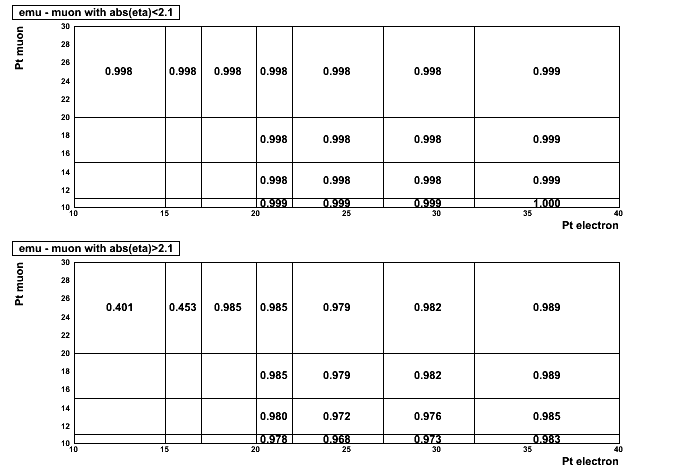
\includegraphics[width=0.99\linewidth]{emuModel.png}
\caption{\label{fig:emuModel}\protect Trigger efficiency for the
$e\mu$ pair as a function of the $P_T$ of the two leptons.
The top table corresponds to $|\eta(\mu)| < 2.1$, the bottom
table to $|\eta(\mu)| > 2.1$.} 
\end{center}
\end{figure}
\clearpage


\begin{figure}[tbh]
\begin{center}
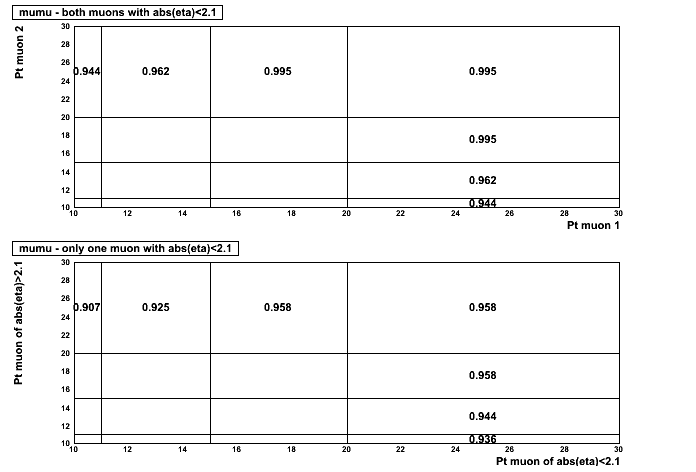
\includegraphics[width=0.99\linewidth]{mumuModel.png}
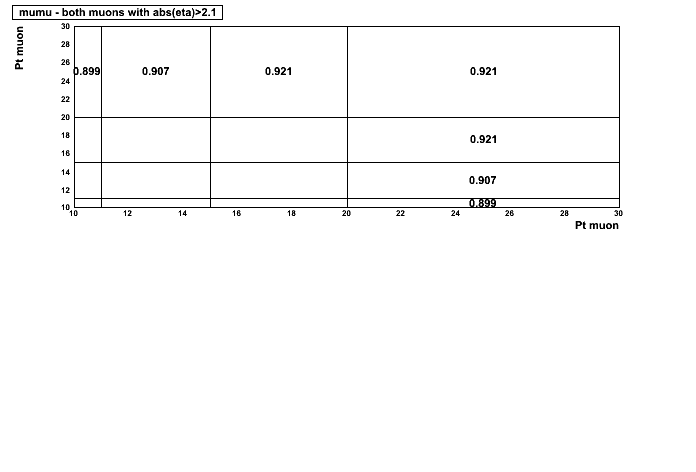
\includegraphics[width=0.99\linewidth]{mumu24Model.png}
\caption{\label{fig:mumuModel}\protect Trigger efficiency for the
$\mu\mu$ pair as a function of the $P_T$ of the two muons.
The top table corresponds to both muons having $|\eta| < 2.1$;
the middle table has one of the muon with $|\eta|<2.1$ and the
other muon with $|\eta|>2.1$; the bottom table has both muons with 
have $|\eta|>2.1$.}
\end{center}
\end{figure}

\clearpage

\subsection{$e\mu$ trigger study}
\label{sec:emutrg}
The $e\mu$ cross triggers were introduced late in the run and are
not well studied (as far as we know).  We performed a study to verify 
the key assumptions of the model:
\begin{enumerate}
\item the $\mu$ component of the $e\mu$ trigger is at least as efficient
as the single muon trigger; 
\item the electron component of the $e\mu$ trigger is essentially 100\% efficient,
as already determined by tag and probe.
\end{enumerate}

To this end, we select $e\mu$ events in the run ranges were the
$e\mu$ triggers were operational as follows:
\begin{itemize}
\item An offline muon of $P_T > 10$ GeV satisfying the standard
requireemnts.
\item This muon must have fired one of the unprescaled single muon triggers.
\item An offline electron of $P_T > 20$ GeV satisfying the standard requirements.
%\item This electron must have fired one of the unprescaled electron triggers,
%which are known to be essentially 100\% efficient on real electrons
%from tag \& probe studies.
\end{itemize}



\begin{figure}[hbt]
\begin{center}
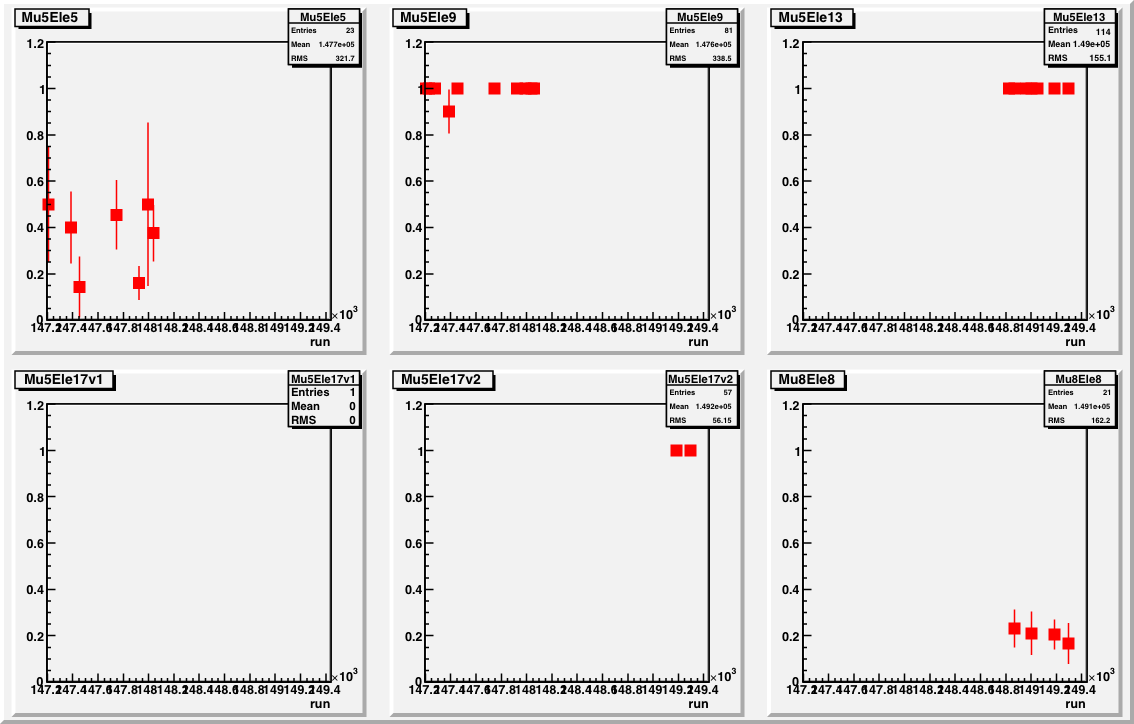
\includegraphics[width=\linewidth]{emu_trigger.png}
\caption{\label{fig:emutrg}\protect $e\mu$ trigger efficiency
as a function of run number.  We plot the trigger 
efficiency of a given variant of the $e\mu$ trigger only for
the runs when said trigger was enabled.} 
\end{center}
\end{figure}


We then defined the $e\mu$ trigger efficiency as the probability
for $e\mu$ trigger to fire on these events.
The results are shown in Figure~\ref{fig:emutrg}.  We find 100\%
trigger efficiency (as expected) for {\tt Mu5\_Ele9}, {\tt Mu5\_Ele13},
and {\tt Mu5\_Ele17\_V2}.  The other triggers ({\tt Mu5\_Ele5},
{\tt Mu8\_Ele8}, and {\tt Mu5\_Ele17\_V1}) do not work very well.  
We note that the working triggers are seeded at L1 by both Mu and EG.
On the other hand, {\tt Mu5\_Ele5} and {\tt Mu8\_Ele8} are only seeded
by Mu. We have since learned\cite{ref:harper} that the inefficiency
of these triggers is due to an HLT bug that has recently been understood.
The source of inefficiency of {\tt Mu5\_Ele17\_V1}
is not understood
at the moment.  Nevertheless, the working $e\mu$ triggers safely 
cover the run ranges with the problematic $e\mu$ triggers.

Thus, our key trigger model assumptions are verified, {\em i.e.}, the
muon trigger piece of the $e\mu$ trigger is at least as efficient 
as the single muon trigger, and the electron piece is essentially
100\% efficient.

%Note that if we calculate the efficiency
%relaxing the requirement on the single electron trigger, we find
%$e\mu$ trigger efficiencies of order 90\% instead of 100\% (for the 
%working set of triggers).  This must be due to the fact that we
%are measuring the efficiency on ``junk'' electrons, and the 
%electron trigger efficiency on these electrons is not exactly
%100\% (the tag \& probe efficiency measurement on electrons from 
%$Z \to ee$ gives essentially 100\%).
   %\setcounter{table}{0}
\renewcommand\thetable{\Alph{section}.\arabic{table}}
\setcounter{figure}{0}
\renewcommand\thefigure{\Alph{section}.\arabic{figure}}
\section{Anatomy of the candidate event}
\label{sec:cand}
The candidate event is an $e\mu + 3$ jets event (run=148864, lumi=225,
event=267767817).  A summary of the objects in the event is given in
Table~\ref{tab:cand1}; event displays are in Figure~\ref{fig:cand1}.

The {\tt ParticleFlow} and {\tt tcMet/JPT} reconstructions of
jets and \met are very consistent. The event shows a clear back
to back topology, as would be expected from a $t\bar{t}$ event
with high $M(t\bar{t})$ (but any statement on the origin of this
event is just a speculation, of course).

\begin{table}[htb]
\begin{center}
\caption{\label{tab:cand1} Summary of the objects in the candidate event.}
\begin{tabular}{|l|c|c|c|c|c|}
\hline
               &  $P_T$ (GeV) & $\eta$  &  $\phi$  &  b-tagged? & value \\ \hline
muon           &   136.       &  0.046  &  -0.206  &            &       \\
electron       &    88        &  0.389  &   2.529  &            &       \\ \hline
Jet 1 (jpt)    &   267        & -0.161  &   2.709  &  Y         &       \\
Jet 2 (jpt)    &    42        &  0.786  &  -0.739  &  N         &       \\
Jet 3 (jpt)    &    40        &  0.192  &  -1.025  &  N         &       \\ 
SumJetPt (jpt) &              &         &          &            & 350 GeV   \\ \hline
Jet 1  (pf)    &   263        & -0.165  &   2.709  &  Y         &       \\
Jet 2  (pf)    &    49        &  0.727  &  -0.723  &  N         &       \\
Jet 3  (pf)    &    34        &  0.117  &  -1.020  &  N         &       \\ 
SumJetPt  (pf) &              &         &          &            & 347 GeV   \\ \hline
tcMET          &   198        &         &  -0.557  &            &       \\ 
pfMET          &   194        &         &  -0.503  &            &       \\ \hline
$P_T(\ell\ell)$&    65        &         &   0.354  &            &       \\
$M(\ell\ell)$  &              &         &          &            & 217 GeV \\
MT2 (tcMet)    &              &         &          &            & 42 GeV  \\
MT2J (tc$+$JPT)&              &         &          &            & 97 GeV  \\
Mass (tc$+$JPT)&              &         &          &            & 159 GeV \\
Meff (tc$+$JPT)&              &         &          &            & 771 GeV \\
\hline
\end{tabular}
\end{center}
\end{table}


\begin{figure}[tbh]
\begin{center}
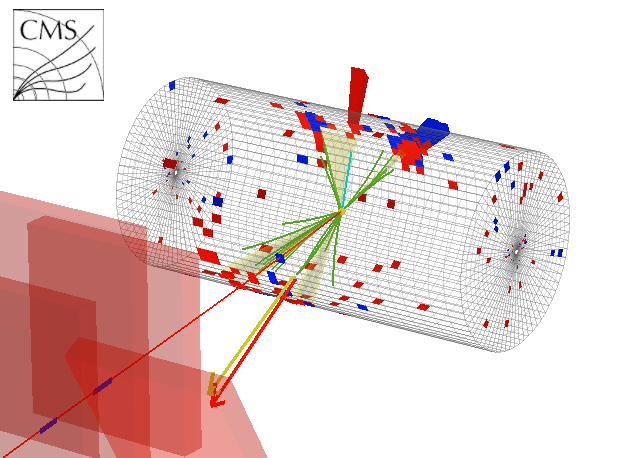
\includegraphics[width=0.6\linewidth]{OSG_3D.png}
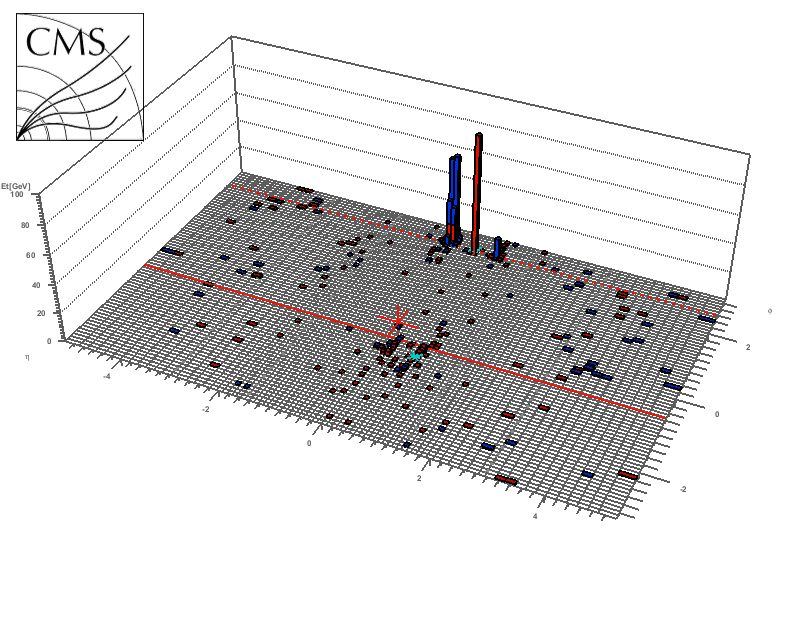
\includegraphics[width=0.6\linewidth]{OSG_lego.png}
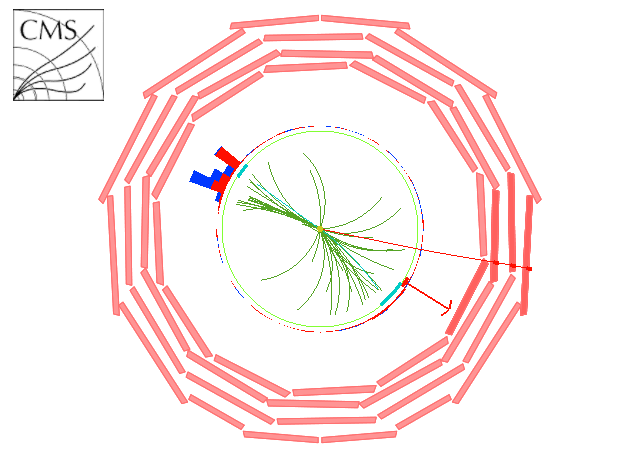
\includegraphics[width=0.6\linewidth]{OSG_rphi.png}
\caption{\label{fig:cand1}Event display for the candidate event.}
\end{center}
\end{figure}

\clearpage

   %\section{Comparison of data and MC distributions}
\label{sec:appendix}
Here we compare data and MC distributions for data passing the 
preselection requirements.  In some cases, {\em e.g.} the 
\met distribution, we show the ``$N-1$ plot'', {\em i.e.}, the 
plot for the variable with all other kinematical cuts
applied except the cut on the variable itself.  The
cut value is then indicated by a vertical red dashed line.

The meaning of most of the variables plotted in 
the following figures should be obvious.  There
are some exceptions that we exlain below

\begin{itemize}

\item $MT2$ in Figure C29 is a kinematical quantity 
built from the two leptons and the \met.  For events with
two $W \to \ell$ decays it should have a sharp kinematical cutoff
at $W$ mass.  For more details, see Reference~\cite{ref:MT2}.

\item $MT2J$ in Figure C30 is very muck like $MT2$ but it is built 
out of the leptons the \met and the two jets.  For $t\bar{t}$
events it has a kinematical cutoff at $M_{\rm top}$, with tails
due to the fact that occasionally one of the $b$-jets is not
found and is replaced by a gluon jet from ISR or FSR.
For more details, see Reference~\cite{ref:MT2J}.

\item The reconstructed top mass in Figure C6 is from the 
kinematical mass reconstruction of the top dilepton group.
In this case we are using the $D0$ matrix-element technique.
See Reference~\cite{ref:brown} for more details.

\end{itemize}


\clearpage

%\includepdf[pages=-, landscape=true, turn=false, offset=0mm -20mm]{datamc_ossusy.pdf}
%\includepdf[pages=-, landscape=true, turn=false, offset=0mm -20mm]{datamc_ossusy_oct15.pdf}

%Removed several plots temporarily (3rd and 4th jet pt, eta, btag info, mt)
%\includepdf[pages=-, landscape=true, turn=false, offset=0mm -20mm]{datamc_35pb.pdf}
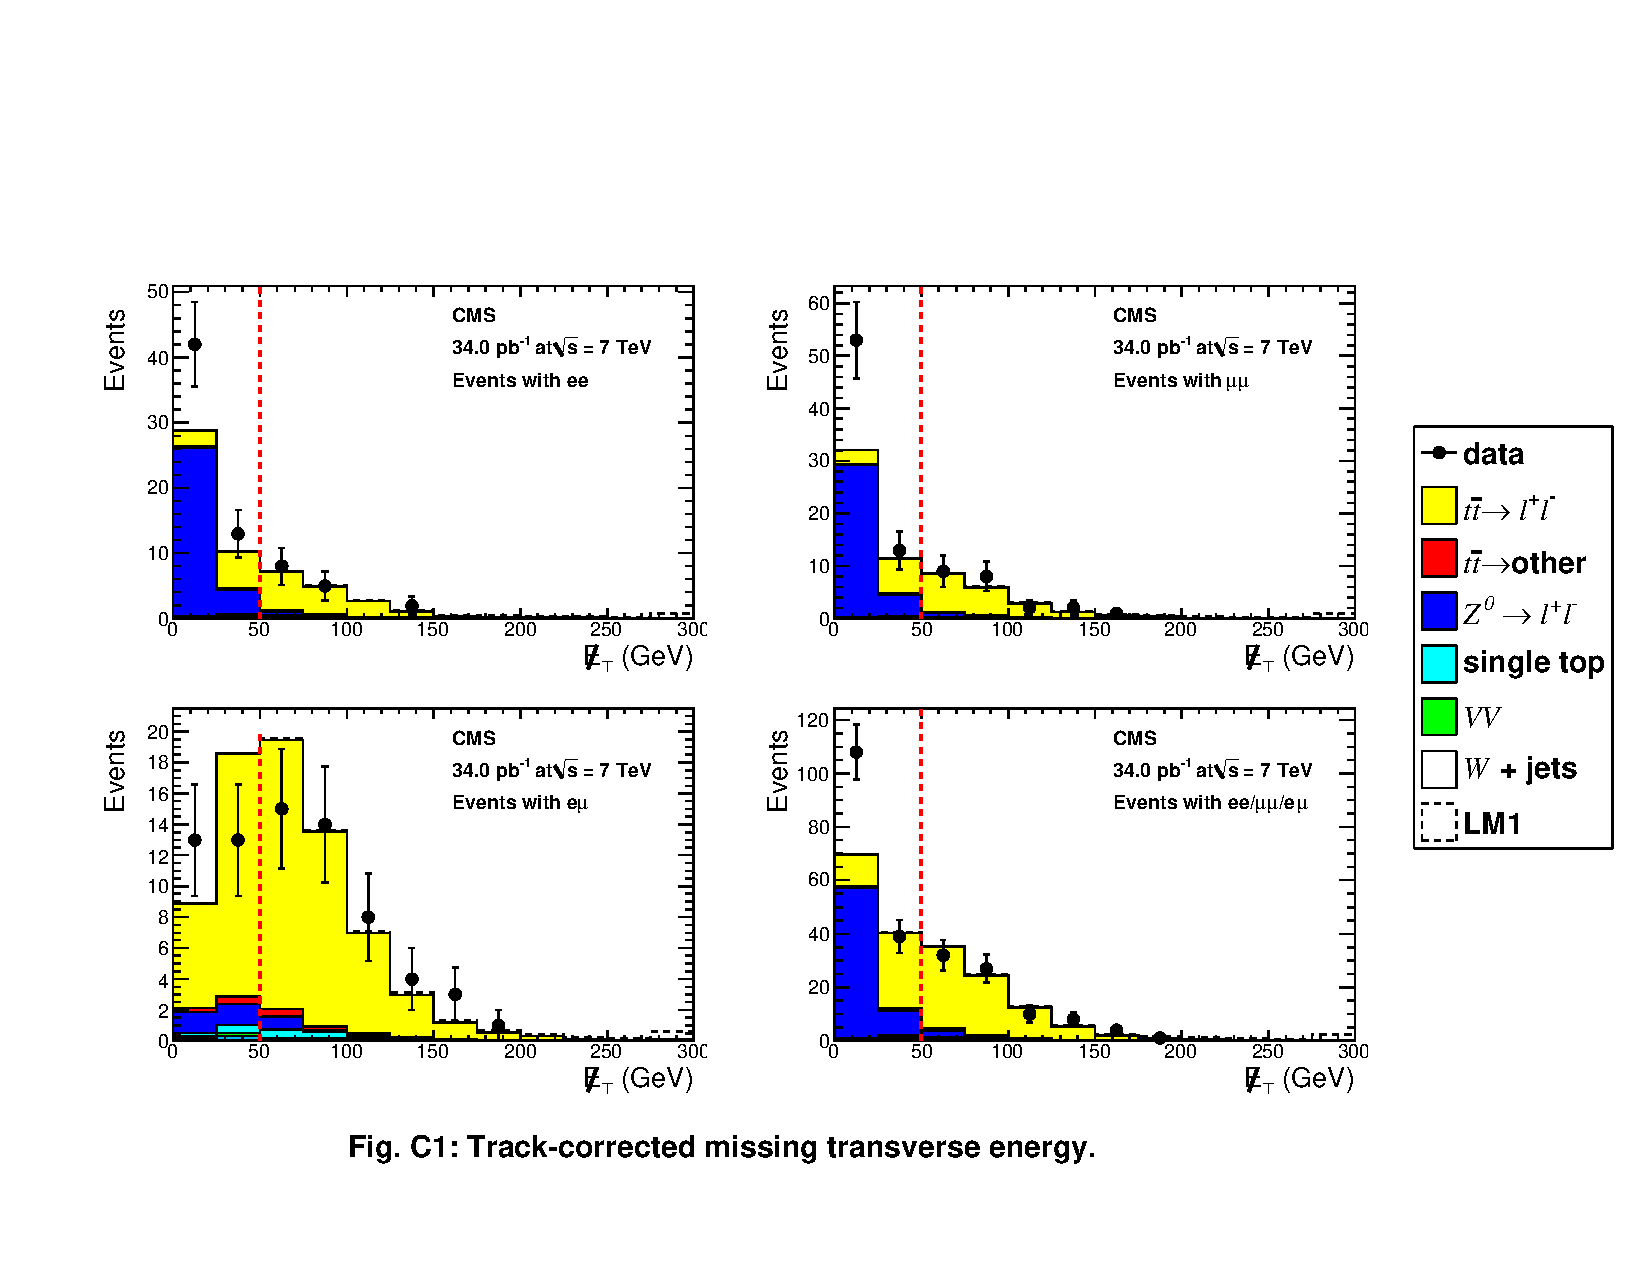
\includepdf[pages=-, landscape=true, turn=false, offset=0mm -20mm]{datamc_v3.pdf}
\end{appendices}
% \setcounter{page}{2}%JPP





\end{document}
